% Groundwater Audit from Space -- research report and software design
% Compile: pdflatex main.tex (twice)
\documentclass[11pt,a4paper]{article}
\usepackage[T1]{fontenc}
\usepackage[utf8]{inputenc}
\usepackage[sc]{mathpazo}
\usepackage[scaled=0.92]{helvet}
\renewcommand{\ttdefault}{lmtt}
\usepackage{microtype}
\usepackage[a4paper,left=24mm,right=24mm,top=25mm,bottom=25mm]{geometry}
\usepackage{amsmath,amssymb}
\usepackage[table]{xcolor}
\usepackage{graphicx}
\usepackage{booktabs,tabularx,longtable,array,makecell}
\usepackage{xltabular}
\usepackage{needspace}
\usepackage{enumitem}
\usepackage{titlesec}
\usepackage{fancyhdr}
\usepackage[most]{tcolorbox}
\usepackage{tikz}
\usetikzlibrary{arrows.meta,positioning,shapes.geometric,fit,calc,backgrounds}
\usepackage{pgf-umlsd}
\usepackage{caption}
\usepackage{float}
\usepackage[hidelinks]{hyperref}
\usepackage{xurl}

% ---------- colours ----------
\definecolor{ink}{HTML}{10232B}
\definecolor{muted}{HTML}{52514E}
\definecolor{accent}{HTML}{1C5CAB}
\definecolor{accentsoft}{HTML}{E6EFFA}
\definecolor{warm}{HTML}{B4491E}
\definecolor{warmsoft}{HTML}{FCEDE6}
\definecolor{green}{HTML}{0F7A55}
\definecolor{greensoft}{HTML}{E4F4EE}
\definecolor{line}{HTML}{C9D3D8}
\definecolor{rowalt}{HTML}{F4F7F9}
\color{ink}
\hypersetup{colorlinks=true,linkcolor=accent,urlcolor=accent,citecolor=accent}

% ---------- traceability tags (\textcircled) ----------
% One letter says what kind of thing it is, the circled number says which one.
\newcommand{\cir}[1]{\textcircled{\raisebox{-0.9pt}{\scriptsize\sffamily\bfseries #1}}}
\newcommand{\trtag}[3]{\mbox{\textcolor{#1}{\sffamily\bfseries #2\kern0.8pt\cir{#3}}}}
\newcommand{\Q}[1]{\trtag{accent}{Q}{#1}}   % research question
\newcommand{\D}[1]{\trtag{green}{D}{#1}}    % data set
\newcommand{\M}[1]{\trtag{warm}{M}{#1}}     % method stage
\newcommand{\V}[1]{\trtag{accent}{V}{#1}}   % validation check
\newcommand{\R}[1]{\trtag{warm}{R}{#1}}     % risk
\newcommand{\U}[1]{\trtag{green}{U}{#1}}    % user need
\newcommand{\Sx}[1]{\trtag{accent}{S}{#1}}  % software component
\newcommand{\Ox}[1]{\trtag{green}{O}{#1}}   % output

% ---------- headings ----------
\titleformat{\part}[display]{\sffamily\bfseries\Huge\color{accent}}{\large Part \thepart}{6pt}{}
\titleformat{\section}{\sffamily\bfseries\Large\color{ink}}{\thesection}{0.7em}{}
\titleformat{\subsection}{\sffamily\bfseries\large\color{ink}}{\thesubsection}{0.6em}{}
\titleformat{\subsubsection}{\sffamily\bfseries\normalsize\color{accent}}{}{0em}{}
\titlespacing*{\section}{0pt}{16pt}{6pt}
\titlespacing*{\subsection}{0pt}{12pt}{4pt}
\titlespacing*{\subsubsection}{0pt}{9pt}{2pt}
\setlength{\parindent}{0pt}
\setlength{\parskip}{6pt}
\setlist{itemsep=2pt,topsep=3pt,leftmargin=1.5em}
\renewcommand{\arraystretch}{1.25}
\captionsetup{font={small,sf},labelfont=bf,skip=6pt}
\setlength{\LTcapwidth}{\linewidth}\setlength{\LTpre}{8pt}\setlength{\LTpost}{8pt}

\setlength{\headheight}{14pt}
\pagestyle{fancy}
\fancyhf{}
\fancyhead[L]{\small\sffamily\color{muted}Groundwater Audit from Space}
\fancyhead[R]{\small\sffamily\color{muted}\nouppercase{\leftmark}}
\fancyfoot[C]{\small\sffamily\color{muted}\thepage}
\renewcommand{\headrulewidth}{0.3pt}
\renewcommand{\headrule}{\color{line}\hrule width\headwidth height\headrulewidth}

% ---------- boxes ----------
\newtcolorbox{inshort}{enhanced,breakable,colback=accentsoft,colframe=accentsoft,boxrule=0pt,arc=2pt,
  left=10pt,right=10pt,top=7pt,bottom=7pt,borderline west={3pt}{0pt}{accent},
  before upper={\textsf{\textbf{\color{accent}In short.}}\ }}
\newtcolorbox{plain}{enhanced,breakable,colback=greensoft,colframe=greensoft,boxrule=0pt,arc=2pt,
  left=10pt,right=10pt,top=7pt,bottom=7pt,borderline west={3pt}{0pt}{green},
  before upper={\textsf{\textbf{\color{green}In plain words.}}\ }}
\newtcolorbox{caution}{enhanced,breakable,colback=warmsoft,colframe=warmsoft,boxrule=0pt,arc=2pt,
  left=10pt,right=10pt,top=7pt,bottom=7pt,borderline west={3pt}{0pt}{warm},
  before upper={\textsf{\textbf{\color{warm}Honest limit.}}\ }}
\newcommand{\trace}[1]{\par{\small\sffamily\color{muted}\textbf{Trace:} #1}\par}

% ---------- small helpers ----------
\newcommand{\kcm}{$\times10^{3}$\,m$^{3}$/yr}
\newcommand{\mmyr}{mm/yr}
\newcolumntype{L}[1]{>{\raggedright\arraybackslash}p{#1}}
\newcolumntype{Y}{>{\raggedright\arraybackslash}X}
\tikzset{
  box/.style={draw=line,fill=white,rounded corners=2pt,align=center,font=\sffamily\small,inner sep=5pt,text=ink},
  boxa/.style={box,draw=accent,fill=accentsoft},
  boxg/.style={box,draw=green,fill=greensoft},
  boxw/.style={box,draw=warm,fill=warmsoft},
  arr/.style={-{Stealth[length=5pt]},draw=muted,line width=0.6pt},
  lab/.style={font=\sffamily\scriptsize,text=muted}
}

% generated by code/analyze.py -- do not edit
\newcommand{\calRecall}{89}
\newcommand{\calPrecision}{80}
\newcommand{\calMedErr}{7}
\newcommand{\calLoc}{59}
\newcommand{\calTot}{0.97}
\newcommand{\calTotMin}{0.75}
\newcommand{\calTotMax}{1.12}
\newcommand{\calNest}{162}
\newcommand{\calTp}{130}
\newcommand{\calErrNinety}{32}
\newcommand{\cvRecall}{88}
\newcommand{\cvPrecision}{78}
\newcommand{\cvMedErr}{23}
\newcommand{\cvLoc}{67}
\newcommand{\cvTot}{1.02}
\newcommand{\cvTotMin}{0.64}
\newcommand{\cvTotMax}{2.30}
\newcommand{\cvNest}{165}
\newcommand{\cvTp}{129}
\newcommand{\cvErrNinety}{90}
\newcommand{\smRecall}{90}
\newcommand{\smPrecision}{35}
\newcommand{\smMedErr}{15}
\newcommand{\smLoc}{197}
\newcommand{\smTot}{1.18}
\newcommand{\smTotMin}{0.87}
\newcommand{\smTotMax}{2.83}
\newcommand{\smNest}{377}
\newcommand{\smTp}{131}
\newcommand{\smErrNinety}{39}
\newcommand{\boRecall}{28}
\newcommand{\boPrecision}{89}
\newcommand{\boMedErr}{81}
\newcommand{\boLoc}{115}
\newcommand{\boTot}{0.11}
\newcommand{\boTotMin}{0.03}
\newcommand{\boTotMax}{0.30}
\newcommand{\boNest}{46}
\newcommand{\boTp}{41}
\newcommand{\boErrNinety}{89}
\newcommand{\nScen}{20}
\newcommand{\nTrue}{146}
\newcommand{\noiseSd}{2.1}
\newcommand{\calCover}{85}
\newcommand{\cvCover}{77}
\newcommand{\calRecallStab}{84}
\newcommand{\calPrecisionStab}{92}
\newcommand{\calFp}{32}
\newcommand{\calFpStab}{10}
\newcommand{\calStabTp}{0.93}
\newcommand{\calStabFp}{0.71}
\newcommand{\cvBexact}{8}
\newcommand{\cvBnear}{16}
\newcommand{\cvBmin}{1.25}
\newcommand{\cvBmax}{2.50}
\newcommand{\cvGoodErr}{7}
\newcommand{\cvBadErr}{35}
\newcommand{\recallSmall}{86}
\newcommand{\nSmall}{43}
\newcommand{\recallMid}{92}
\newcommand{\nMid}{39}
\newcommand{\recallLarge}{89}
\newcommand{\nLarge}{64}
\newcommand{\totNarrow}{0.43}
\newcommand{\recNarrow}{61}
\newcommand{\precNarrow}{84}
\newcommand{\totOneK}{0.52}
\newcommand{\recOneK}{85}
\newcommand{\precOneK}{89}
\newcommand{\totTwoK}{1.43}
\newcommand{\recTwoK}{86}
\newcommand{\precTwoK}{68}
\newcommand{\totWide}{2.08}
\newcommand{\recWide}{86}
\newcommand{\precWide}{54}
\newcommand{\totGaussOne}{0.47}
\newcommand{\recGaussOne}{81}
\newcommand{\precGaussOne}{87}
\newcommand{\totGaussMid}{0.92}
\newcommand{\recGaussMid}{69}
\newcommand{\precGaussMid}{89}
\newcommand{\totGaussTwo}{1.35}
\newcommand{\recGaussTwo}{44}
\newcommand{\precGaussTwo}{76}
\newcommand{\noiseHalf}{1.1}
\newcommand{\recNHalf}{93}
\newcommand{\precNHalf}{90}
\newcommand{\errNHalf}{7}
\newcommand{\noiseBase}{2.1}
\newcommand{\recNBase}{92}
\newcommand{\precNBase}{82}
\newcommand{\errNBase}{7}
\newcommand{\noiseTwo}{4.3}
\newcommand{\recNTwo}{90}
\newcommand{\precNTwo}{65}
\newcommand{\errNTwo}{8}
\newcommand{\noiseThree}{6.4}
\newcommand{\recNThree}{85}
\newcommand{\precNThree}{62}
\newcommand{\errNThree}{10}
\newcommand{\noiseFour}{8.5}
\newcommand{\recNFour}{79}
\newcommand{\precNFour}{58}
\newcommand{\errNFour}{14}
\newcommand{\resHalf}{0}
\newcommand{\resThreeQ}{12}
\newcommand{\resOne}{62}
\newcommand{\resOneHalf}{75}
\newcommand{\resTwo}{100}
\newcommand{\resThree}{88}
\newcommand{\rankCal}{0.94}
\newcommand{\rankCv}{0.94}
\newcommand{\rankNarrow}{0.89}
\newcommand{\rankOneK}{0.89}
\newcommand{\rankTwoK}{0.88}
\newcommand{\rankWide}{0.86}
\newcommand{\tabEtwo}{%
1.1 & 93 & 90 & 7 & 0.99\\
2.1 & 92 & 82 & 7 & 1.03\\
4.3 & 90 & 65 & 8 & 1.03\\
6.4 & 85 & 62 & 10 & 1.07\\
8.5 & 79 & 58 & 14 & 1.16\\}
\newcommand{\tabEthree}{%
0.5 & 0.75 & 0 of 8 & 1.11\\
0.75 & 1.12 & 1 of 8 & 1.10\\
1 & 1.50 & 5 of 8 & 1.09\\
1.5 & 2.25 & 6 of 8 & 1.11\\
2 & 3.00 & 8 of 8 & 1.14\\
3 & 4.50 & 7 of 8 & 1.16\\}
\newcommand{\tabEfour}{%
Bessel (true family) & 0.75 & 61 & 84 & 56 & 0.43\\
Bessel (true family) & 1.00 & 85 & 89 & 41 & 0.52\\
Bessel (true family) & 1.25 & 86 & 85 & 21 & 0.70\\
Bessel (true family) & 1.50 (true) & 86 & 78 & 6 & 0.91\\
Bessel (true family) & 2.00 & 86 & 68 & 58 & 1.43\\
Bessel (true family) & 2.50 & 86 & 54 & 132 & 2.08\\
\midrule
Gaussian (wrong family) & 1.00 & 81 & 87 & 42 & 0.47\\
Gaussian (wrong family) & 1.50 & 69 & 89 & 24 & 0.92\\
Gaussian (wrong family) & 2.00 & 44 & 76 & 108 & 1.35\\}


\begin{document}
% ===================== Executive summary: two pages, visual first =====================
\newgeometry{left=22mm,right=22mm,top=15mm,bottom=17mm}
\fancypagestyle{execfoot}{\fancyhf{}\renewcommand{\headrulewidth}{0pt}\renewcommand{\headrule}{}\fancyfoot[C]{\small\sffamily\color{muted}\thepage}}
\thispagestyle{empty}\phantomsection\addcontentsline{toc}{section}{Executive summary}
\markboth{Executive summary}{Executive summary}
\definecolor{claycol}{HTML}{EFE4D6}
\definecolor{sandcol}{HTML}{DCE9F8}
\definecolor{deepcol}{HTML}{E3E7EA}
% section label with a pointer to the full section
\newcommand{\xhead}[2]{\par\vspace{2.2mm}\noindent
  {\sffamily\bfseries\small\color{accent}\MakeUppercase{#1}}\hfill{\sffamily\scriptsize\color{muted}#2}\\[-7pt]
  {\color{line}\rule{\linewidth}{0.5pt}}\par\vspace{0.6mm}}
\newcommand{\xyes}{\textcolor{green}{\large\checkmark}}
\newcommand{\xno}{\textcolor{line}{\rule[2pt]{9pt}{1.2pt}}}
\newcommand{\xpart}{\textcolor{muted}{\sffamily\scriptsize partly}}
\tcbset{tile/.style={enhanced,colback=#1,colframe=#1,boxrule=0pt,arc=2pt,left=7pt,right=7pt,top=6pt,bottom=6pt,
  fontupper=\sffamily\footnotesize\raggedright}}
\newcommand{\tilebig}[2]{{\sffamily\bfseries\fontsize{19}{21}\selectfont\color{#1}#2}\\[2pt]}

\begin{center}
{\sffamily\scriptsize\color{muted} ASEAN Geospatial Challenge 2027 \textbullet\ National Level: Indonesia \textbullet\ working document, 16 November 2026}\\[3mm]
{\sffamily\bfseries\fontsize{24}{27}\selectfont\color{ink} Groundwater Audit from Space}\\[2mm]
{\sffamily\large\color{accent} Tracing land subsidence in Semarang--Demak back to the pumping that causes it}
\end{center}
\vspace{-1mm}

\begin{tcolorbox}[enhanced,colback=accent,colframe=accent,boxrule=0pt,arc=2pt,left=10pt,right=10pt,top=7pt,bottom=7pt]
\sffamily\color{white}\textbf{Executive summary.} Satellites already show \emph{where} the coast of Central Java
is sinking. This project works out \emph{which pumping causes it, and how much}: a ranked list of
groundwater extraction hot spots, each with a volume and an error bar, made without a well registry.
\end{tcolorbox}

% ---------------------------------------------------------------- PROBLEM
\xhead{The problem}{Sections \ref{sec:problem}--\ref{sec:area}}
\begin{tcbraster}[raster columns=3,raster equal height,raster column skip=3mm,raster before skip=1mm,raster after skip=0mm]
\begin{tcolorbox}[tile=warmsoft]
\tilebig{warm}{14\,cm a year}
The fastest sinking measured in Semarang and Demak, 2020--2023 \cite{janur2025}. Tidal floods (\emph{rob}) keep getting worse.
\end{tcolorbox}
\begin{tcolorbox}[tile=warmsoft]
\tilebig{warm}{2010}
The last year with usable well records. By then more than 1,000 deep wells were pumping
\cite{lo2022,putranto2016}.
\end{tcolorbox}
\begin{tcolorbox}[tile=warmsoft]
\tilebig{warm}{Which wells?}
Permits exist, but nobody can say which pumping does the damage. Inspectors have no list to
start from.
\end{tcolorbox}
\end{tcbraster}

% ---------------------------------------------------------------- IDEA
\xhead{The idea: pumping leaves a fingerprint on the ground}{Section \ref{sec:physics}}
\noindent
\begin{minipage}[c]{0.59\linewidth}
\begin{tikzpicture}[x=1cm,y=1.22cm,font=\sffamily\scriptsize]
  \def\surf{(0,3.5) .. controls (2.2,3.5) and (3.0,3.1) .. (4.3,3.1) .. controls (5.6,3.1) and (6.4,3.5) .. (8.6,3.5) -- (9.6,3.5)}
  % layers
  \fill[deepcol] (0,0) rectangle (9.6,0.5);
  \fill[sandcol] (0,0.5) rectangle (9.6,1.7);
  \fill[claycol] (0,1.7) -- \surf -- (9.6,1.7) -- cycle;
  % old and new surface
  \draw[muted,dash pattern=on 2pt off 2pt,line width=0.4pt] (0,3.5) -- (9.6,3.5);
  \draw[ink,line width=0.9pt] \surf;
  % layer names
  \node[anchor=east,text=muted] at (9.5,2.17) {clay};
  \node[anchor=east,text=muted] at (9.5,0.95) {aquifer: sand and water};
  % pressure level before and after
  \draw[accent,dash pattern=on 2pt off 2pt,line width=0.5pt] (0,2.72) -- (9.6,2.72);
  \draw[accent,line width=1.1pt] (0,2.66) .. controls (2.6,2.62) and (3.7,2.3) .. (4.3,1.0)
       .. controls (4.9,2.3) and (6.0,2.62) .. (9.6,2.66);
  \node[anchor=west,text=accent] at (0.1,2.93) {pressure before pumping};
  % well and factory
  \draw[ink,line width=1.2pt] (4.3,3.1) -- (4.3,0.85);
  \fill[ink] (4.0,3.1) rectangle (4.8,3.38);
  \fill[ink] (4.0,3.38) -- (4.0,3.58) -- (4.27,3.38) -- (4.27,3.58) -- (4.54,3.38) -- (4.54,3.58) -- (4.8,3.38) -- cycle;
  \draw[accent,-{Stealth[length=4pt]},line width=0.9pt] (4.4,3.72) -- (4.4,4.15);
  % compaction arrows
  \foreach \x in {2.3,2.8,5.9,6.4} \draw[warm,-{Stealth[length=3pt]},line width=0.8pt] (\x,2.38) -- (\x,1.95);
  % sinking arrow
  \draw[ink,-{Stealth[length=3pt]},line width=0.7pt] (5.75,3.5) -- (5.75,3.24);
  % satellites
  \foreach \sx/\tx in {1.3/3.2,8.3/5.4}{
    \draw[muted,dash pattern=on 1.5pt off 1.5pt,line width=0.4pt] (\sx,5.1) -- (\tx,3.25);
    \fill[ink] (\sx-0.16,5.03) rectangle (\sx+0.16,5.23);
    \fill[accent] (\sx-0.62,5.08) rectangle (\sx-0.2,5.18);
    \fill[accent] (\sx+0.2,5.08) rectangle (\sx+0.62,5.18);
  }
  \node[text=muted] at (4.8,5.13) {radar satellite, two viewing directions};
  % step tags
  \node[anchor=west,text=ink] at (4.52,4.0) {\textcolor{accent}{\cir{1}} pumping};
  \node[anchor=west,text=accent] at (4.75,1.2) {\cir{2} pressure cone};
  \node[anchor=west,text=warm] at (0.1,2.17) {\cir{3} clay compacts};
  \node[anchor=west,text=ink] at (5.9,3.74) {\cir{4} ground sinks};
\end{tikzpicture}
\end{minipage}\hfill
\begin{minipage}[c]{0.37\linewidth}\sffamily\footnotesize\raggedright
\textcolor{accent}{\cir{1}} A deep well pumps water out.\\[2.5pt]
\textcolor{accent}{\cir{2}} Water pressure falls in a cone several kilometres wide.\\[2.5pt]
\textcolor{warm}{\cir{3}} Clay drains and compacts. Most of this is permanent.\\[2.5pt]
\cir{4} The ground sinks in the same cone shape. Radar measures it from space.\\[5pt]
\begin{tcolorbox}[tile=greensoft,left=6pt,right=6pt,top=5pt,bottom=5pt]
\textbf{\color{green}We read the chain backwards}, from \cir{4} to \cir{1}. The shape of each
bowl tells us where the pumping sits and how much storage is lost there.
\end{tcolorbox}
\end{minipage}

% ---------------------------------------------------------------- SOLUTION
\xhead{The solution: from a sinking map to an audit list}{Section \ref{sec:exp}}
\begin{center}
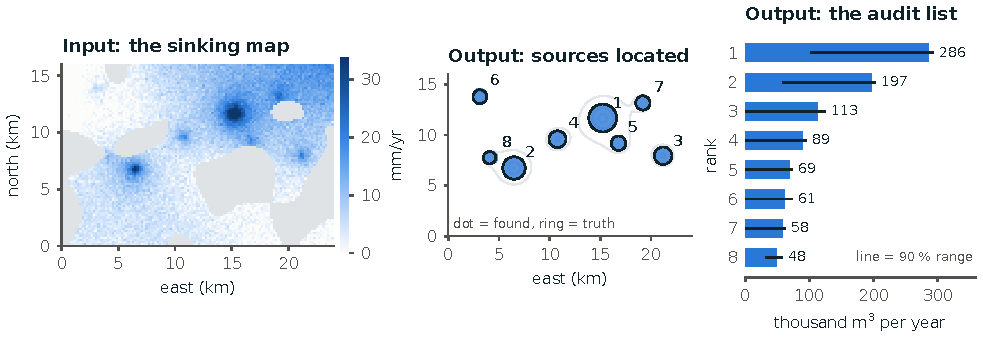
\includegraphics[width=\linewidth]{fig/exec_solution.pdf}
\end{center}
\vspace{-3mm}
{\sffamily\scriptsize\color{muted} One of \nScen\ simulated test maps, with the noise and data gaps of real radar. Eight sources
were hidden; the method found all eight and ranked them. Volume means storage lost by the aquifer, a
lower bound on water pumped. A run on real Semarang data is the next step (Section~\ref{sec:spike}).\par}

\clearpage\thispagestyle{execfoot}
% ======================================================================= PAGE 2
% ---------------------------------------------------------------- METHOD
\xhead{The method in three moves}{Sections \ref{sec:method}--\ref{sec:rigour}}
\noindent
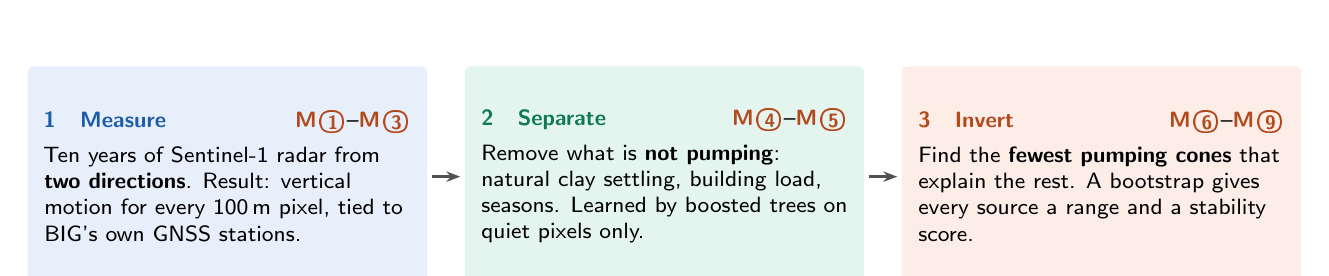
\begin{tikzpicture}[font=\sffamily\footnotesize]
  \tikzset{card/.style={rounded corners=2pt,text width=46.5mm,minimum height=28mm,align=flush left,inner sep=6pt,anchor=north west}}
  \node[card,fill=accentsoft] (a) at (0,0) {%
    {\bfseries\color{accent}1\quad Measure}\hfill\M{1}--\M{3}\\[3pt]
    Ten years of Sentinel-1 radar from \textbf{two directions}. Result: vertical motion for every
    100\,m pixel, tied to BIG's own GNSS stations.};
  \node[card,fill=greensoft] (b) at (55.5mm,0) {%
    {\bfseries\color{green}2\quad Separate}\hfill\M{4}--\M{5}\\[3pt]
    Remove what is \textbf{not pumping}: natural clay settling, building load, seasons. Learned
    by boosted trees on quiet pixels only.};
  \node[card,fill=warmsoft] (c) at (111mm,0) {%
    {\bfseries\color{warm}3\quad Invert}\hfill\M{6}--\M{9}\\[3pt]
    Find the \textbf{fewest pumping cones} that explain the rest. A bootstrap gives every source a
    range and a stability score.};
  \draw[arr,line width=0.9pt] ($(a.east)+(0.5mm,0)$) -- ($(b.west)+(-0.5mm,0)$);
  \draw[arr,line width=0.9pt] ($(b.east)+(0.5mm,0)$) -- ($(c.west)+(-0.5mm,0)$);
\end{tikzpicture}

\vspace{1mm}
{\sffamily\footnotesize\color{ink}\textbf{Why it is rigorous.} A physics model sits inside the learning step, so every
number has a unit. Splits are spatial blocks, never random pixels. Each learned part has a baseline
to beat and a pass mark set in advance (\V{1}--\V{7}).\par}

% ---------------------------------------------------------------- EVIDENCE
\xhead{The evidence so far}{Section \ref{sec:exp}}
\noindent
\begin{minipage}[t]{0.56\linewidth}\vspace{0pt}
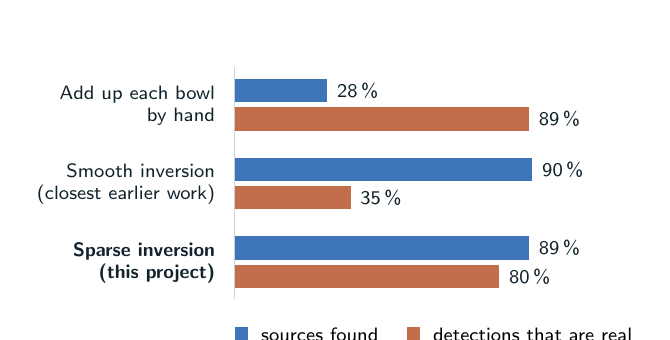
\begin{tikzpicture}[x=0.42mm,y=1mm,font=\sffamily\scriptsize]
  % x from 0 to 100 (%), label column to the left
  \def\barrow#1#2#3#4{% y, label, recall, precision
    \node[anchor=east,align=right,text=ink] at (-3,#1+2.6) {#2};
    \fill[accent!85] (0,#1+3.0) rectangle (#3,#1+6.0);
    \fill[warm!80] (0,#1-0.6) rectangle (#4,#1+2.4);
    \node[anchor=west,text=ink] at (#3,#1+4.5) {#3\,\%};
    \node[anchor=west,text=ink] at (#4,#1+0.9) {#4\,\%};
  }
  \draw[line] (0,-2.0) -- (0,27.5);
  \barrow{20}{Add up each bowl\\by hand}{\boRecall}{\boPrecision}
  \barrow{10}{Smooth inversion\\(closest earlier work)}{\smRecall}{\smPrecision}
  \barrow{0}{\textbf{Sparse inversion}\\\textbf{(this project)}}{\calRecall}{\calPrecision}
  \fill[accent!85] (0,-7.5) rectangle (4,-5.5); \node[anchor=west] at (5,-6.5) {sources found};
  \fill[warm!80] (52,-7.5) rectangle (56,-5.5); \node[anchor=west] at (57,-6.5) {detections that are real};
\end{tikzpicture}
\end{minipage}\hfill
\begin{minipage}[t]{0.41\linewidth}\vspace{0pt}\sffamily\footnotesize\raggedright
\textbf{\nScen\ simulated maps, \nTrue\ hidden sources.} Only the sparse inversion both finds the
sources and avoids false alarms.\\[5pt]
\begin{tabular}{@{}>{\bfseries\fontsize{15}{17}\selectfont\color{accent}}r@{\hspace{7pt}}L{43mm}@{}}
\calMedErr\,\% & median volume error, when the cone width is known\\[2pt]
\calLoc\,m & median position error\\[2pt]
\calCover\,\% & of true volumes fall inside the stated 90\,\% range\\
\end{tabular}
\end{minipage}

\vspace{1mm}
\begin{tcolorbox}[tile=warmsoft,left=8pt,right=8pt,top=4pt,bottom=3pt]
\begin{minipage}[c]{0.47\linewidth}\raggedright
\textbf{\color{warm}The honest limit: one number we cannot see from space.}
Volumes depend on the width of a pumping cone. Guess it wrong and every volume shifts together.
The \emph{order} of the list barely moves.
\end{minipage}\hfill
\begin{minipage}[c]{0.50\linewidth}
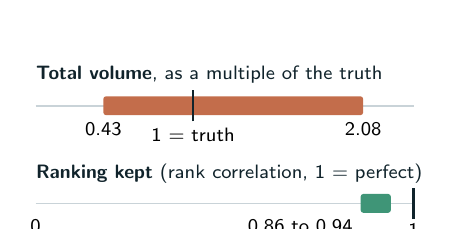
\begin{tikzpicture}[x=20mm,y=1mm,font=\sffamily\scriptsize]
  \node[anchor=west,text=ink,inner sep=0pt] at (0,9.3) {\textbf{Total volume}, as a multiple of the truth};
  \draw[line,line width=0.6pt] (0,5.4) -- (2.4,5.4);
  \fill[warm!80,rounded corners=1pt] (\totNarrow,4.2) rectangle (\totWide,6.6);
  \draw[ink,line width=0.9pt] (1,3.4) -- (1,7.4);
  \node[anchor=north,inner sep=1pt] at (\totNarrow,3.6) {\totNarrow};
  \node[anchor=north,inner sep=1pt] at (1,3.0) {1 = truth};
  \node[anchor=north,inner sep=1pt] at (\totWide,3.6) {\totWide};
  \node[anchor=west,text=ink,inner sep=0pt] at (0,-3.2) {\textbf{Ranking kept} (rank correlation, 1 = perfect)};
  \draw[line,line width=0.6pt] (0,-7.0) -- (2.4,-7.0);
  \fill[green!80,rounded corners=1pt] (\rankWide*2.4,-8.2) rectangle (\rankCal*2.4,-5.8);
  \draw[ink,line width=0.9pt] (2.4,-9.0) -- (2.4,-5.0);
  \node[anchor=north,inner sep=1pt] at (0,-8.6) {0};
  \node[anchor=north east,inner sep=1pt] at (\rankWide*2.4-0.03,-8.6) {\rankWide\ to \rankCal};
  \node[anchor=north,inner sep=1pt] at (2.4,-9.2) {1};
\end{tikzpicture}
\end{minipage}
\end{tcolorbox}

% ---------------------------------------------------------------- UVP
\xhead{What makes it different}{Section \ref{sec:prior}}
{\sffamily\footnotesize
\noindent\begin{tabularx}{\linewidth}{@{}L{56mm}*{5}{>{\centering\arraybackslash}X}@{}}
 & \textbf{No registry needed} & \textbf{Short list of sources} & \textbf{Volume per source} & \textbf{Error bar per source} & \textbf{Natural part removed}\\
\midrule
Subsidence maps \cite{abidin2013,aditiya2023,janur2025} & \xyes & \xno & \xno & \xno & \xno\\
Groundwater flow model \cite{lo2022} & \xno & \xno & \xno & \xno & \xpart\\
Smooth inversion, Semarang 2025 \cite{azeriansyah2025} & \xyes & \xno & \xpart & \xno & \xno\\
\rowcolor{accentsoft}\textbf{This project} & \xyes & \xyes & \xyes & \xyes & \xyes\\
\bottomrule
\end{tabularx}}

\vspace{0.5mm}
{\sffamily\scriptsize\color{muted} Closest precedent abroad: a California study guided by a public well registry \cite{vasco2019}. Our ticks are shown in simulation so far.\par}

% ---------------------------------------------------------------- WHY IT CAN WIN
\xhead{Why it can win}{Section \ref{sec:plan}}
\noindent
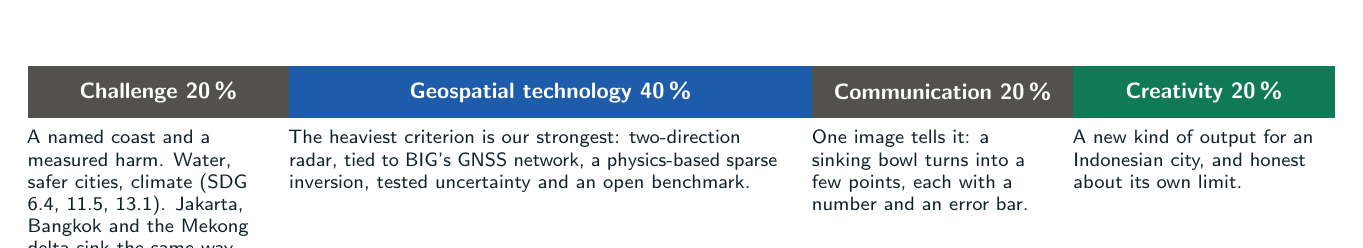
\begin{tikzpicture}[font=\sffamily\scriptsize]
  \tikzset{seg/.style={minimum height=6.5mm,inner sep=0pt,anchor=west,text=white,font=\sffamily\bfseries\fontsize{7.6}{9}\selectfont},
           why/.style={anchor=north west,align=flush left,inner sep=0pt,text=ink}}
  \node[seg,fill=muted,minimum width=33.2mm] (s1) at (0,0) {Challenge 20\,\%};
  \node[seg,fill=accent,minimum width=66.4mm] (s2) at (33.2mm,0) {Geospatial technology 40\,\%};
  \node[seg,fill=muted,minimum width=33.2mm] (s3) at (99.6mm,0) {Communication 20\,\%};
  \node[seg,fill=green,minimum width=33.2mm] (s4) at (132.8mm,0) {Creativity 20\,\%};
  \node[why,text width=30mm] at ($(s1.south west)+(0,-1.5mm)$) {A named coast and a measured harm. Water, safer cities, climate (SDG 6.4, 11.5, 13.1). Jakarta, Bangkok and the Mekong delta sink the same way.};
  \node[why,text width=62mm] at ($(s2.south west)+(0,-1.5mm)$) {The heaviest criterion is our strongest: two-direction radar, tied to BIG's GNSS network, a physics-based sparse inversion, tested uncertainty and an open benchmark.};
  \node[why,text width=30mm] at ($(s3.south west)+(0,-1.5mm)$) {One image tells it: a sinking bowl turns into a few points, each with a number and an error bar.};
  \node[why,text width=30.5mm] at ($(s4.south west)+(0,-1.5mm)$) {A new kind of output for an Indonesian city, and honest about its own limit.};
\end{tikzpicture}

% ---------------------------------------------------------------- STATUS
\xhead{Where it stands}{Section \ref{sec:feas}}
\begin{tcbraster}[raster columns=3,raster equal height,raster column skip=3mm,raster before skip=1mm,raster after skip=0mm]
\begin{tcolorbox}[tile=greensoft]
\textbf{\color{green}Proven by others}\\[1pt]
Measuring Semarang's sinking with this satellite: four published studies.
\end{tcolorbox}
\begin{tcolorbox}[tile=accentsoft]
\textbf{\color{accent}Works in simulation}\\[1pt]
Finding, ranking and sizing sources, with ranges that hold up.
\end{tcolorbox}
\begin{tcolorbox}[tile=warmsoft]
\textbf{\color{warm}Not done yet}\\[1pt]
A run on real Semarang data: one week, four pass marks (Section~\ref{sec:spike}).
\end{tcolorbox}
\end{tcbraster}
\clearpage
\restoregeometry

\section*{About this document}
\markboth{About this document}{About this document}

\textbf{Assumptions made for this document.} Study area: Semarang--Demak. Team: four students with one
radar specialist. Time: six weeks. Change any of these and the method stays; only
Sections~\ref{sec:data} and~\ref{sec:feas} need updating.

\subsection*{How to read this document}

Every item that matters has a tag: a letter for its kind and a circled number. Tags let you follow
one thread through the whole document. For example, \Q{2} (which sources?) is answered by stage \M{6},
checked by \V{3}, built in component \Sx{4}, and delivered as output \Ox{3}. Section~\ref{sec:trace}
lists every such link.

\begin{center}
\small\renewcommand{\arraystretch}{1.0}
\begin{tabular}{@{}llp{62mm}l@{}}
\toprule
\textbf{Tag} & \textbf{Kind} & \textbf{Meaning} & \textbf{Defined in}\\*
\midrule
\Q{1}--\Q{3} & Question & What the research must answer & Section 2\\
\D{1}--\D{9} & Data & A data set and where it comes from & Section~\ref{sec:data}\\
\M{1}--\M{9} & Method & One stage of the pipeline & Section~\ref{sec:method}\\
\V{1}--\V{7} & Validation & A check with a pass mark & Section~\ref{sec:rigour}\\
\R{1}--\R{8} & Risk & What could go wrong, and the response & Section~\ref{sec:feas}\\
\U{1}--\U{6} & User need & What a user must be able to do & Section~\ref{sec:product}\\
\Sx{1}--\Sx{9} & Software & A component of the system & Section~\ref{sec:arch}\\
\Ox{1}--\Ox{5} & Output & Something the project delivers & Section 2\\
\bottomrule
\end{tabular}
\end{center}

Three kinds of boxes recur. \textcolor{accent}{\textsf{\textbf{In short}}} gives the point of a
section. \textcolor{green}{\textsf{\textbf{In plain words}}} explains an idea without jargon.
\textcolor{warm}{\textsf{\textbf{Honest limit}}} says what a result does not show.

\enlargethispage{2\baselineskip}
{\sffamily\footnotesize\hypersetup{linkcolor=ink}\setcounter{tocdepth}{1}\setlength{\parskip}{0pt}\makeatletter\renewcommand*\l@section{\@dottedtocline{1}{0em}{2.2em}}\makeatother\tableofcontents}
\clearpage

\clearpage\part{Research report}
\section{The idea on one page}

\begin{inshort}
Satellites already show \emph{where} the ground in Semarang--Demak is sinking. This project asks the
next question: \emph{which groundwater extraction sources cause it, and how much water does each one
take from storage?} The result is a ranked list of extraction hot spots, each with a volume and an
error bar, that a regulator could act on.
\end{inshort}

\textbf{Why it matters.} Sinking land is the main reason tidal floods (\emph{rob}) keep getting worse on
Java's north coast. Parts of Semarang and Demak sink by more than 10\,cm a year
\cite{aditiya2023,janur2025}. Pumping from deep wells is a leading cause, but well records are
incomplete, so nobody can say which sources matter most.

\textbf{What we do, in three steps.}
\begin{enumerate}
\item \textbf{Measure.} Process ten years of Sentinel-1 radar images from two viewing directions into
      maps of vertical ground motion, tied to BIG's GNSS stations.
\item \textbf{Separate.} Split the motion into a pumping part and a non-pumping part (natural settling
      of young clay, weight of buildings), and into long-term and seasonal behaviour.
\item \textbf{Invert.} Find the smallest set of extraction sources that explains the pumping part.
      Each source gets a location, a volume of lost storage per year, and an uncertainty range.
\end{enumerate}

\textbf{What is new.} Earlier work in Semarang mapped the sinking and fitted smooth source models.
None of it produced a short, ranked list of sources with uncertainty, and none linked the result to
extraction volumes. A similar idea was shown in California, where a well registry guided the
inversion \cite{vasco2019}. We do it where no reliable registry exists.

\textbf{What this report already proves.} We built the inversion and tested it on a synthetic copy of
the problem (Section~\ref{sec:exp}). With the cone width known, it found \calRecall\,\% of the
hidden sources with \calPrecision\,\% precision, and estimated their volumes with a median error of
\calMedErr\,\%. Two standard alternatives did clearly worse. The test also exposed the method's
weakest point: volumes depend on one hydrogeological parameter (the width of a pumping cone) that
radar alone cannot pin down. Section~\ref{sec:feas} turns that into a concrete plan.

\textbf{What is still open.} The method has not yet been run on real Semarang data. Section~\ref{sec:spike}
defines a one-week test with clear pass and fail criteria.

\section{Problem and research questions}\label{sec:problem}

Indonesia regulates groundwater use through permits. Since 2023, even households that use more than
100\,m$^3$ a month need approval \cite{kepmen291}, and the energy ministry lists Semarang among the
areas with serious groundwater damage \cite{esdm2023}. Permits only help if someone can check them.
Today the checking tools are flow meters, where they are installed, and a sparse set of monitoring
wells.

\begin{plain}
Pumping water out of deep sand layers lowers the water pressure. The clay layers around the sand then
get squeezed, like a wet sponge under a weight, and the ground above sinks. Most of that squeezing is
permanent. So sinking ground is a physical record of pumping, and radar satellites can read it.
\end{plain}

The project answers three research questions. Their tags are used throughout the document.

\begin{tabularx}{\linewidth}{@{}L{12mm}Y@{}}
\toprule
\Q{1} & \textbf{Measurement.} How fast is the ground moving, vertically and east--west, at about
        100\,m resolution, and how certain is each value?\\
\Q{2} & \textbf{Attribution.} Which extraction sources explain the pumping-driven sinking, and how much
        storage volume does each one remove per year?\\
\Q{3} & \textbf{Separation.} How much of the sinking is \emph{not} caused by pumping, and how confident
        can we be in that split?\\
\bottomrule
\end{tabularx}

The answers are delivered as five outputs.

\begin{tabularx}{\linewidth}{@{}L{12mm}Y L{24mm}@{}}
\toprule
 & \textbf{Output} & \textbf{Answers}\\*
\midrule
\Ox{1} & Maps of vertical and east--west velocity with uncertainty & \Q{1}\\
\Ox{2} & Maps of seasonal amplitude and of dates when the motion changed & \Q{1} \Q{3}\\
\Ox{3} & Ranked list of extraction hot spots: location, volume, 90\,\% range, stability & \Q{2}\\
\Ox{4} & Map of non-pumping (background) subsidence & \Q{3}\\
\Ox{5} & Audit report and interactive web map & \Q{1} \Q{2} \Q{3}\\
\bottomrule
\end{tabularx}

\Needspace{17\baselineskip}
\section{Study area: Semarang--Demak}\label{sec:area}

Semarang is the capital of Central Java. Its northern half and neighbouring Demak lie on a young
coastal plain of soft clay and sand. Table~\ref{tab:area} lists what published work says about it.

\Needspace{8\baselineskip}
{\small
\begin{xltabular}{\linewidth}{@{}L{34mm}Y L{20mm}@{}}
\caption{What is known about the study area. Each row names its source.}\label{tab:area}\\*
\toprule
\textbf{Topic} & \textbf{Finding} & \textbf{Source}\\*
\midrule
Sinking rate, 2008--2011 & GPS surveys: 6--7\,cm/yr on average, up to 14--19\,cm/yr in places. Faster in the
  north, near the coast. & \cite{abidin2013}\\
Sinking rate, 2015--2022 & Radar: up to 100--120\,mm/yr in north and east Semarang and Demak. About 20\,\% of
  the city's land is affected. Deformation correlates with groundwater (coefficient 0.86). & \cite{aditiya2023}\\
Sinking rate, 2020--2023 & Radar from two directions: highest vertical rates of about 144\,mm/yr (Semarang) and
  146\,mm/yr (Demak). Vertical error against 12 GNSS stations: 8.8\,mm. & \cite{janur2025}\\
Causes & Natural settling of young alluvial soil, groundwater extraction, and the load of buildings. & \cite{abidin2013}\\
Aquifers & One unconfined aquifer and a confined system with three groups (Garang, Quaternary marine, Damar),
  separated by clay layers 5--30\,m thick. & \cite{putranto2016}\\
Well depths & Deep wells tap the confined Damar aquifer at 60--180\,m. The Genuk district draws from 60--120\,m
  and is classed as a critical zone. & \cite{lo2022,aghnia2022}\\
Extraction history & First deep well in 1841; 16 wells by 1900; more than 1,000 wells and over
  30 million m$^3$/yr by 2010. Records stop in 2010. & \cite{putranto2016,lo2022}\\
Sustainable yield & The confined aquifer is credited with about 16.5 million m$^3$/yr, well below the 30 million
  or more that is pumped. & \cite{frontiers2023}\\
Water pressure & The confined water level fell 0.7--1.1\,m per year, to about 20\,m below sea level. & \cite{fahrudin2012}\\
Tectonic motion & Small: 3--5\,mm/yr of regional subsidence in GNSS data. & \cite{lo2022}\\
\bottomrule
\end{xltabular}}

Two details in this table motivate the project. First, the official well records end in 2010, so any
recent picture of extraction has to come from somewhere else. Second, a groundwater model driven by
those records reproduces at most 36.8\,mm/yr of sinking in Genuk, while radar from 2015--2020 shows
more than 80\,mm/yr in the same part of the city \cite{lo2022}. The periods differ, so this is not
proof, but it suggests that recorded pumping does not tell the whole story.

\Needspace{14\baselineskip}
\section{Prior work and the gap}\label{sec:prior}

\Needspace{8\baselineskip}
{\small
\begin{xltabular}{\linewidth}{@{}L{31mm}Y Y@{}}
\caption{The closest earlier studies and what each leaves open.}\label{tab:prior}\\*
\toprule
\textbf{Study} & \textbf{What it did} & \textbf{What it leaves open}\\*
\midrule
Chaussard et al.\ 2013 \cite{chaussard2013} & Mapped sinking in Indonesian cities with ALOS radar. Linked
  fast, patchy sinking to industrial land. & A visual link only. No source volumes.\\
Lo et al.\ 2022 \cite{lo2022} & Groundwater-flow and compaction model (MODFLOW) for Semarang, checked against
  radar. & Needs well records as input, and those end in 2010.\\
Aditiya \& Ito 2023 \cite{aditiya2023} & Radar time series 2015--2022 with GNSS support. & A motion map. No
  sources.\\
Azeriansyah et al.\ 2025 \cite{azeriansyah2025} & Inverted one radar track into volume loss on a 250\,m grid of
  point sources at a fixed depth of 120\,m, with smoothing. & The result is a smooth map, not a list of sources.
  No uncertainty per source, no link to pumping, and east--west motion is predicted, not measured.\\
Janur et al.\ 2025 \cite{janur2025} & Two-direction radar along the whole north coast, checked against GNSS. &
  A motion map. No sources.\\
Vasco et al.\ 2019 \cite{vasco2019} & California: inverted radar for aquifer volume change, steering the
  solution towards registered wells. Stated the volumes are lower bounds on extraction. & Relies on a public
  well registry. Blocks of 2\,km. No sparse source list.\\
\bottomrule
\end{xltabular}}

\textbf{The gap.} Nobody has yet produced, for an Indonesian city, a short list of extraction sources
with volumes and uncertainty, built without relying on a well registry.

\textbf{Our four contributions.}
\begin{enumerate}
\item A \emph{sparse} inversion that returns few, well-separated sources instead of a smooth map
      (stage \M{6}).
\item A source model based on how a pumping cone spreads in a leaky aquifer, not only on elastic
      point sources. Section~\ref{sec:identity} shows why the elastic model alone carries almost no
      information about sources at these depths.
\item Honest uncertainty for every source: a 90\,\% range and a stability score (stage \M{7}), with the
      penalty level set from the data's own noise.
\item An explicit, testable split between pumping and non-pumping subsidence (stage \M{5}).
\end{enumerate}

\Needspace{16\baselineskip}
\section{Data}\label{sec:data}

Every data set has a tag. The last column says how sure we are that the team can get it.

\Needspace{8\baselineskip}
{\small
\begin{xltabular}{\linewidth}{@{}L{9mm}L{33mm}Y L{27mm}@{}}
\caption{Data inventory.}\label{tab:data}\\*
\toprule
 & \textbf{Data set} & \textbf{Details and source} & \textbf{Access}\\*
\midrule
\D{1} & Sentinel-1 radar & C-band, 2015 to now, two directions: descending track 76 (ready-made LiCSAR frame
  \texttt{076D\_09725\_121107} \cite{lo2022}) and ascending track 127 (confirm in ASF Vertex). & Open\\
\D{2} & NISAR radar & L-band, sees through vegetation better. Calibrated products are public for images
  from 17 June 2026; earlier images are being reprocessed during 2026 \cite{nisar2026}. & Open, short record\\
\D{3} & GACOS & Maps of radar delay in the lower atmosphere, used for correction \cite{yu2018}. & Open, on request\\
\D{4} & InaCORS GNSS & BIG's permanent stations, including CSEM in Semarang, through the SRGI portal. & Request to BIG\\
\D{5} & Elevation model & DEMNAS from BIG, or the Copernicus 30\,m model. & Open\\
\D{6} & Groundwater records & Monitoring-well water levels, conservation-zone map and well permits from the
  Geological Agency and the Central Java energy office. & Request, uncertain\\
\D{7} & Geology & Borehole logs, hydrogeological map, thickness of soft clay \cite{putranto2016}. & Partly published\\
\D{8} & Buildings and land use & Building footprints (Google Open Buildings, OpenStreetMap), built-up volume
  (GHSL), industrial estates. & Open\\
\D{9} & Rainfall and tides & CHIRPS rainfall; BIG tide gauges. Used to explain seasonal signals. & Open / request\\
\bottomrule
\end{xltabular}}

\textbf{Satellite status (November 2026).} Sentinel-1A ended operations on 29 June 2026 after twelve
years. Sentinel-1C (data since March 2025) and Sentinel-1D (data since April 2026) now give a 6-day
repeat \cite{s1status}. Sentinel-1B failed in December 2021, so 2022--2024 has one image every
12 days. The series is continuous enough for our purpose, but the processing must handle the change
of satellites.

\textbf{What is essential.} Only \D{1}, \D{3}, \D{5} and \D{8} are needed to run the whole pipeline, and
all four are open. \D{4} makes the motion maps trustworthy. \D{6} is what turns a good map into a
validated audit; if it cannot be obtained in time, the report says so and relies on checks
\V{1}--\V{4} (Section~\ref{sec:rigour}).

\section{How the physics works}\label{sec:physics}

\begin{inshort}
Pumping creates a cone of low water pressure around a well field. Clay inside that cone compacts, and
the ground above sinks in the same cone-shaped pattern. Our inversion reads that pattern backwards.
\end{inshort}

\begin{figure}[H]
\centering
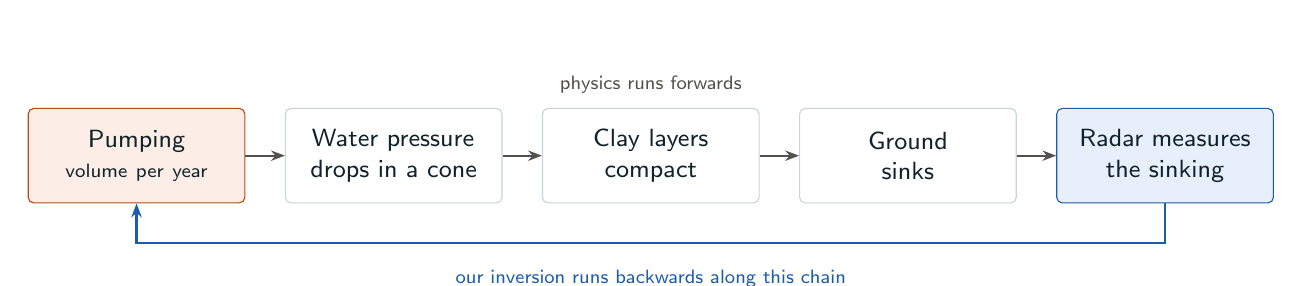
\begin{tikzpicture}[node distance=5mm]
\tikzset{ch/.style={box,text width=24mm,minimum height=12mm}}
\node[ch,boxw] (a) {Pumping\\{\scriptsize volume per year}};
\node[ch,right=of a] (b) {Water pressure\\drops in a cone};
\node[ch,right=of b] (c) {Clay layers\\compact};
\node[ch,right=of c] (d) {Ground\\sinks};
\node[ch,boxa,right=of d] (e) {Radar measures\\the sinking};
\draw[arr] (a)--(b); \draw[arr] (b)--(c); \draw[arr] (c)--(d); \draw[arr] (d)--(e);
\draw[arr,draw=accent,line width=0.9pt] (e.south) -- ++(0,-5mm) -| (a.south);
\node[lab,text=accent] at ($(c.south)+(0,-9.5mm)$) {our inversion runs backwards along this chain};
\node[lab] at ($(c.north)+(0,3mm)$) {physics runs forwards};
\end{tikzpicture}
\caption{The causal chain. Each arrow is one piece of physics described below.}
\end{figure}

\subsection{From water pressure to compaction}

When the water level (head) $h$ in an aquifer system falls, a layer of thickness $b_0$ compacts by
\begin{equation}
\Delta b \;=\; S_k\,\Delta h, \qquad
S_k = \begin{cases} S_{ke} & \text{if } h \text{ is above its lowest past level (elastic, recoverable)}\\
                    S_{kv} & \text{if } h \text{ falls below it (inelastic, permanent)} \end{cases}
\label{eq:compaction}
\end{equation}
where $S_k$ is the skeletal storage coefficient. $S_{kv}$ is typically one to two orders of magnitude
larger than $S_{ke}$ \cite{galloway2011}. This is why over-pumping is so damaging: once head falls
below its historical minimum, compaction jumps and most of it never recovers. In Semarang, the Damar
aquifer's head has already dropped below that threshold \cite{lo2022}.

Thick clay drains slowly. A clay layer of thickness $b'$, vertical conductivity $K'_v$ and specific
storage $S'_s$ needs a time of the order of
\begin{equation}
\tau \;=\; \frac{(b'/2)^2\,S'_s}{K'_v}
\end{equation}
to adjust \cite{galloway2011}. For metres of clay this is years to decades. Two consequences follow.
The ground keeps sinking long after pumping stabilises, and it sinks in the place where the pressure
cone sits. The second point is what makes attribution possible.

\subsection{Why an elastic point source is not enough}\label{sec:identity}

The usual model for inverting ground motion is a point source of volume change $\Delta V$ at depth
$d$ in an elastic half-space (the Mogi model \cite{mogi1958,geertsma1973}). Its vertical surface
motion at horizontal distance $r$ is
\begin{equation}
u_z(r) \;=\; \frac{(1-\nu)\,\Delta V}{\pi}\;\frac{d}{(r^2+d^2)^{3/2}},
\label{eq:mogi}
\end{equation}
with Poisson's ratio $\nu$. Azeriansyah et al.\ used this model for Semarang with $d = 120$\,m
\cite{azeriansyah2025}. Two short calculations show what it can and cannot tell us.

\textbf{Total volume.} Integrating \eqref{eq:mogi} over the surface gives
$\int u_z\,\mathrm{d}A = 2(1-\nu)\,\Delta V$. The model therefore returns a volume that is simply the
integrated subsidence times a constant.

\textbf{Locality.} The share of a source's surface signal that falls within radius $R$ of it is
\begin{equation}
f(R) \;=\; 1-\frac{d}{\sqrt{R^2+d^2}} .
\end{equation}
For $d = 120$\,m this is 57\,\% within 250\,m and 77\,\% within 500\,m. A source at aquifer depth
moves the ground almost only directly above itself.

\begin{plain}
At a depth of about 100\,m, an elastic point source is nearly a mirror: the inverted ``volume map''
is the subsidence map again, rescaled. It cannot say whether a 3\,km wide bowl comes from one big
well field in the middle or from thirty small wells spread across it. Something else must carry that
information.
\end{plain}

\subsection{The missing piece: the shape of a pumping cone}

That ``something else'' is hydraulics. Around a well field that pumps at rate $Q$ from a confined
aquifer with leaky clay above it, the long-term drawdown is (Hantush and Jacob \cite{hantush1955})
\begin{equation}
s(r) \;=\; \frac{Q}{2\pi T}\;K_0\!\left(\frac{r}{B}\right), \qquad B=\sqrt{\frac{T\,b'}{K'_v}} ,
\label{eq:hantush}
\end{equation}
where $T$ is the aquifer's transmissivity, $K_0$ the modified Bessel function, and $B$ the
\emph{leakage factor}: the distance over which the cone fades. Compaction rate follows drawdown
(Eq.~\ref{eq:compaction}), so each source $j$ at position $\mathbf{x}_j$ adds a cone-shaped piece to
the vertical velocity field:
\begin{equation}
v(\mathbf{x}) \;=\; \sum_{j} q_j\,k_B\big(\lVert\mathbf{x}-\mathbf{x}_j\rVert\big) \;+\; g(\mathbf{x}) \;+\; \varepsilon(\mathbf{x}),
\qquad k_B(r)=\frac{K_0(r/B)}{2\pi B^2}.
\label{eq:model}
\end{equation}
The kernel $k_B$ integrates to one, so $q_j$ is directly the \textbf{compaction volume per year}
caused by source $j$ (m$^3$/yr). $g$ is the non-pumping background, and $\varepsilon$ is measurement
noise. Equation~\eqref{eq:model} is the forward model of this project.

\begin{caution}
The cone shape is a modelling choice. Equation~\eqref{eq:hantush} assumes a uniform aquifer and a
steady cone. Real aquifers are patchy, and $B$ is not known in advance. Section~\ref{sec:exp} measures
how wrong the answers get when the cone shape or width is wrong, and Section~\ref{sec:feas} says how
to calibrate $B$.
\end{caution}

\subsection{From compaction volume to extraction}\label{sec:massbalance}

Pumped water comes from three places: water squeezed out of compacting clay, water released
elastically, and water that leaks in from above or from the sides. Only the first leaves a permanent
mark on the ground. So for every source
\begin{equation}
Q_j \;=\; \frac{q_j}{\varphi_j}, \qquad 0<\varphi_j\le 1 ,
\label{eq:phi}
\end{equation}
where $\varphi_j$ is the share of pumped water that comes from compaction. Because
$\varphi_j \le 1$, \textbf{the compaction volume $q_j$ is a lower bound on extraction}. Vasco et
al.\ reached the same conclusion for California \cite{vasco2019}. With metered wells or head records
(\D{6}), $\varphi$ can be calibrated and the bound becomes an estimate.

\textbf{Order-of-magnitude check.} Suppose 75\,km$^2$ sinks at an average of 5\,cm/yr. (The area is
20\,\% of the city \cite{aditiya2023}; the average rate is our assumption.) That is about
3.7 million m$^3$ of lost storage per year, against more than 30 million m$^3$ pumped
\cite{putranto2016}. This gives $\varphi \approx 0.1$: a plausible value, and a reminder that $q$ is
a conservative number.

\section{Method: nine stages}\label{sec:method}

\begin{figure}[H]
\centering
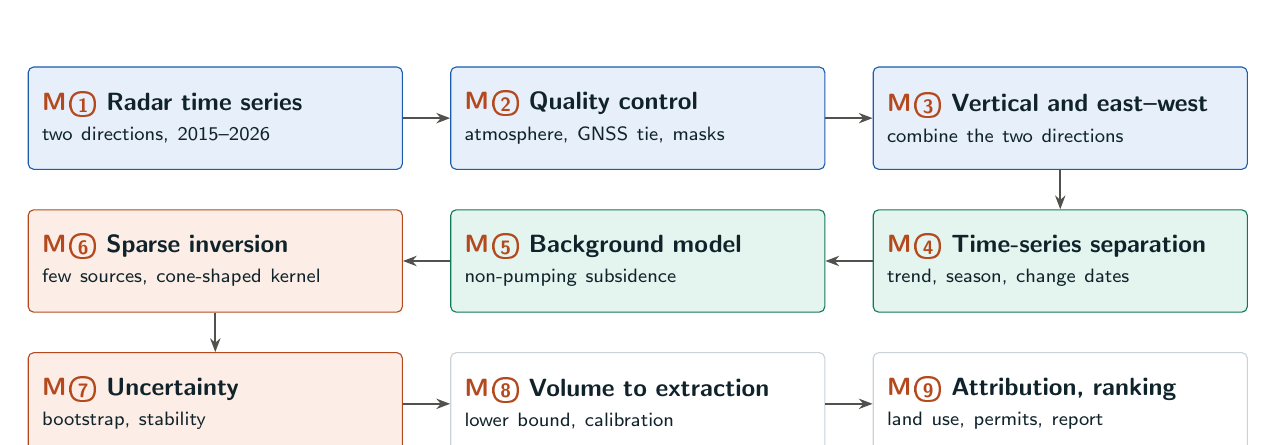
\begin{tikzpicture}[node distance=5mm and 6mm]
\tikzset{st/.style={text width=44mm,minimum height=13mm,align=left}}
\node[boxa,st] (m1) {\M{1} \textbf{Radar time series}\\{\scriptsize two directions, 2015--2026}};
\node[boxa,st,right=of m1] (m2) {\M{2} \textbf{Quality control}\\{\scriptsize atmosphere, GNSS tie, masks}};
\node[boxa,st,right=of m2] (m3) {\M{3} \textbf{Vertical and east--west}\\{\scriptsize combine the two directions}};
\node[boxg,st,below=of m3] (m4) {\M{4} \textbf{Time-series separation}\\{\scriptsize trend, season, change dates}};
\node[boxg,st,left=of m4] (m5) {\M{5} \textbf{Background model}\\{\scriptsize non-pumping subsidence}};
\node[boxw,st,left=of m5] (m6) {\M{6} \textbf{Sparse inversion}\\{\scriptsize few sources, cone-shaped kernel}};
\node[boxw,st,below=of m6] (m7) {\M{7} \textbf{Uncertainty}\\{\scriptsize bootstrap, stability}};
\node[box,st,right=of m7] (m8) {\M{8} \textbf{Volume to extraction}\\{\scriptsize lower bound, calibration}};
\node[box,st,right=of m8] (m9) {\M{9} \textbf{Attribution, ranking}\\{\scriptsize land use, permits, report}};
\draw[arr] (m1)--(m2); \draw[arr] (m2)--(m3); \draw[arr] (m3)--(m4); \draw[arr] (m4)--(m5);
\draw[arr] (m5)--(m6); \draw[arr] (m6)--(m7); \draw[arr] (m7)--(m8); \draw[arr] (m8)--(m9);
\end{tikzpicture}
\caption{The pipeline. Blue: measurement (\Q{1}). Green: separation (\Q{3}). Orange: attribution
(\Q{2}). White: interpretation and delivery.}\label{fig:pipeline}
\end{figure}

\subsubsection{\M{1} Radar time series}
\textbf{What.} Turn stacks of Sentinel-1 images into a displacement history for every pixel.\\
\textbf{How.} Small-baseline (SBAS) processing \cite{berardino2002}: each image is paired with its
next three or four neighbours in time, each pair gives a map of phase change, and a least-squares
solve turns the network of pairs into a time series. For the descending track we start from
ready-made LiCSAR pairs and run LiCSBAS \cite{morishita2020}, as two earlier Semarang studies did
\cite{lo2022,azeriansyah2025}. For the ascending track we order pairs from ASF's on-demand service
and run MintPy \cite{yunjun2019}. Pixels are averaged to about 100\,m. Phase $\phi$ converts to motion
along the line of sight by $d_{\mathrm{LOS}} = -\lambda\phi/4\pi$ with $\lambda = 5.55$\,cm.\\
\textbf{Output.} Two cubes (ascending, descending) of line-of-sight displacement.
\trace{serves \Q{1}; uses \D{1} \D{5}; checked by \V{2}; runs in \Sx{2}.}

\subsubsection{\M{2} Quality control and referencing}
\textbf{What.} Remove what is not ground motion, and fix the zero point.\\
\textbf{How.} (i) Correct the delay from the lower atmosphere with GACOS maps \cite{yu2018}.
(ii) Check \emph{loop closure}: for any three images, the three pairwise phases must sum to zero;
pairs that fail are unwrapping errors and are dropped. (iii) Mask pixels with low coherence
(water, fish ponds, rice fields). (iv) Reference all motion to the CSEM GNSS station, which earlier
work also used \cite{azeriansyah2025}. (v) Estimate a velocity uncertainty per pixel by resampling
the time series.\\
\textbf{Output.} Clean cubes, a validity mask, and a per-pixel uncertainty.
\trace{serves \Q{1}; uses \D{3} \D{4}; checked by \V{1} \V{2}; runs in \Sx{2}.}

\subsubsection{\M{3} Vertical and east--west motion}
\textbf{What.} A single radar direction mixes vertical and horizontal motion. Two directions untangle
them.\\
\textbf{How.} For incidence angle $\theta$ and heading $\alpha$, the line-of-sight unit vector in
(east, north, up) is
\[
\mathbf{l} = (-\sin\theta\cos\alpha,\ \ \sin\theta\sin\alpha,\ \ \cos\theta).
\]
Radar is nearly blind to north--south motion, so we solve per pixel \cite{wright2004}
\begin{equation}
\begin{pmatrix} d^{\mathrm{asc}}\\ d^{\mathrm{desc}}\end{pmatrix} =
\begin{pmatrix} l_E^{\mathrm{asc}} & l_U^{\mathrm{asc}}\\ l_E^{\mathrm{desc}} & l_U^{\mathrm{desc}}\end{pmatrix}
\begin{pmatrix}u_E\\u_U\end{pmatrix}.
\end{equation}
For $\theta \approx 34$--$39^\circ$ the vertical error is about 0.9 times the line-of-sight error and
the east--west error about 1.2 times.\\
\textbf{Output.} Vertical and east--west displacement cubes. East--west motion is a free diagnostic:
ground around a compacting bowl moves inwards.
\trace{serves \Q{1}; produces \Ox{1}; checked by \V{1}; runs in \Sx{4}.}

\subsubsection{\M{4} Time-series separation}
\textbf{What.} Split each pixel's history into long-term trend, seasonal breathing and sudden changes.\\
\textbf{How.} Three tools, from simple to rich.
\begin{itemize}
\item \emph{Robust regression} per pixel:
$u(t) = a + v\,t + c_1\sin 2\pi t + c_2\cos 2\pi t + \varepsilon$, with Huber loss so that outliers
do not bend the trend.
\item \emph{Independent component analysis} (ICA \cite{hyvarinen2000}) on the whole cube, which finds
a few shared time patterns and a map of where each one is strong. It has been used to separate
sources in radar data before \cite{ebmeier2016} and to isolate aquifer signals \cite{chaussard2014}.
\item \emph{Change-point detection} (PELT \cite{killick2012}) on the detrended series, which dates
the moments when sinking sped up or slowed down. A source that switched on or off shows up here.
\end{itemize}
\textbf{Output.} Maps of long-term rate $v$, seasonal amplitude and change dates. The seasonal part
is mostly elastic; a large trend with little seasonal recovery signals permanent compaction
\cite{hoffmann2001,smith2017}.
\trace{serves \Q{1} \Q{3}; produces \Ox{2}; uses \D{9}; checked by \V{4}; runs in \Sx{4}.}

\subsubsection{\M{5} Background model (non-pumping subsidence)}
\textbf{What.} Estimate $g(\mathbf{x})$ in Eq.~\eqref{eq:model}: the sinking that would happen without
deep pumping.\\
\textbf{How.} Two layers.
\begin{itemize}
\item A \emph{driver model}: gradient-boosted trees \cite{chen2016} that predict long-term rate from
soft-clay thickness, land age (reclaimed or not), built-up volume, distance to coast and elevation.
It is trained only on ``quiet'' pixels: those farther than $2B$ from industrial land and from any
known deep well, so that it learns background and not pumping.
\item A \emph{smooth remainder}: a low-order cosine surface that absorbs whatever long-wavelength
signal the drivers miss. It is fitted jointly with the sources in \M{6}.
\end{itemize}
Shapley values (SHAP \cite{lundberg2017}) show which driver matters where.\\
\textbf{Output.} Background map with uncertainty.
\trace{serves \Q{3}; produces \Ox{4}; uses \D{5} \D{7} \D{8}; checked by \V{4}; runs in \Sx{4}.}

\subsubsection{\M{6} Sparse source inversion}
\textbf{What.} Find the few sources $q_j$ that explain the pumping part of the velocity field.\\
\textbf{How.} Lay a grid of candidate source positions $\mathbf{c}_j$ every 500\,m. Build the matrix
$A_{ij}=k_B(\lVert\mathbf{x}_i-\mathbf{c}_j\rVert)$ and a background matrix $Z$ (driver-model
prediction plus cosine surface). Solve
\begin{equation}
\min_{\mathbf{q}\ge 0,\ \boldsymbol\beta}\;\; \frac{1}{2n}\,\big\lVert \mathbf{v}-A\mathbf{q}-Z\boldsymbol\beta\big\rVert_2^2
\;+\;\lambda\sum_j q_j .
\label{eq:lasso}
\end{equation}
This is a non-negative lasso \cite{tibshirani1996}. The constraint $q_j\ge 0$ says sources only
remove volume. The penalty $\lambda\sum q_j$ says: explain the data with as little total volume, in
as few places, as possible. Four details make it trustworthy.
\begin{enumerate}
\item \textbf{Penalty from the data's own noise.} After a first fit we take the residual map, shuffle
its Fourier phases to create 30 fake noise maps with the same spatial texture, and record the
largest source--noise correlation each one produces. $\lambda$ is set no lower than the 95th
percentile of those values. A source then enters only if it stands out from what noise alone could
do.
\item \textbf{Refit without shrinkage.} The lasso picks \emph{where}; a plain non-negative
least-squares refit on the selected positions then estimates \emph{how much}.
\item \textbf{Merging.} Neighbouring selected grid points are merged into one source at their
volume-weighted centre.
\item \textbf{Cone width $B$.} Chosen by spatial cross-validation, or better, fixed from pumping
tests or head data when available (see Section~\ref{sec:exp}).
\end{enumerate}
An optional \emph{informed mode} lowers the penalty for candidates on industrial land, as a soft
version of the well-distance penalty of Vasco et al.\ \cite{vasco2019}. The default \emph{blind mode}
uses no such prior.\\
\textbf{Output.} A source list: position and compaction volume.
\trace{serves \Q{2}; uses output of \M{3}--\M{5}; checked by \V{3} \V{5} \V{6}; runs in \Sx{4}.}

\subsubsection{\M{7} Uncertainty}
\textbf{What.} Say how sure we are of each source.\\
\textbf{How.} A \emph{spatial block bootstrap}: cut the map into 2\,km blocks, resample blocks with
replacement, and rerun the inversion. Repeating this 60--200 times gives, for each source, a 90\,\%
range for its volume and a \emph{stability} score: the share of reruns in which it reappears, in the
spirit of stability selection \cite{meinshausen2010}. Blocks are used because neighbouring pixels
share noise; resampling single pixels would give falsely narrow ranges.\\
\textbf{Output.} Volume range and stability for each source.
\trace{serves \Q{2}; produces \Ox{3}; checked by \V{7}; runs in \Sx{4}.}

\subsubsection{\M{8} From volume to extraction}
\textbf{What.} Translate compaction volume into a statement about pumping.\\
\textbf{How.} Report $q_j$ as a lower bound (Eq.~\ref{eq:phi}). Where metered extraction or head
records exist for some sources, fit $\varphi$ by regression and use it, with its spread, to convert
the other sources into estimated ranges.\\
\textbf{Output.} For each source: minimum extraction, and estimated extraction if calibration data
exist.
\trace{serves \Q{2}; uses \D{6}; checked by \V{5}; runs in \Sx{4}.}

\subsubsection{\M{9} Attribution and ranking}
\textbf{What.} Make the list usable.\\
\textbf{How.} Join each source with land use, building footprints and, if available, the permit
register. Classify it as \emph{matches a permitted well field}, \emph{no permit on record nearby}, or
\emph{unclear}. Rank by volume, then by stability. Public outputs show hot-spot cells, never company
names (Section~\ref{sec:ethics}).\\
\textbf{Output.} The audit list and report.
\trace{serves \Q{2}; produces \Ox{3} \Ox{5}; uses \D{6} \D{8}; checked by \V{6}; runs in \Sx{7} \Sx{9}.}

\section{ML/AI rigour: how we know it works}\label{sec:rigour}

\begin{inshort}
Four parts of the pipeline learn from data. Each has a baseline to beat, a split that prevents
leakage, a metric with a pass mark, and an uncertainty estimate that is itself tested.
\end{inshort}

\Needspace{27\baselineskip}
\subsection{The learning components}

\Needspace{21\baselineskip}
{\small
\begin{xltabular}{\linewidth}{@{}L{8mm}L{33mm}L{30mm}Y@{}}
\toprule
 & \textbf{Component} & \textbf{Type} & \textbf{Why it is not a black box}\\*
\midrule
\M{4} & Trend, season, change dates & Robust regression, ICA, change-point detection & Every output
  is a physical quantity (rate, amplitude, date) that can be checked against GNSS and rainfall.\\
\M{5} & Background driver model & Gradient-boosted trees with SHAP & Trained only on pixels away from
  pumping; each prediction is explained by named drivers.\\
\M{6} & Source inversion & Sparse regression (non-negative lasso) with a physics kernel & Linear and
  convex: one global optimum, every source is a visible term in Eq.~\eqref{eq:model}.\\
\M{7} & Uncertainty & Block bootstrap, stability selection & Ranges are tested for coverage on
  synthetic truth (\V{7}).\\
\bottomrule
\end{xltabular}}

\subsection{Splits and leakage rules}

Map data break the usual assumption that samples are independent: a pixel's neighbours are almost
copies of it. A random train/test split would then report excellent scores for a model that has
learned nothing transferable \cite{roberts2017}. We therefore fix these rules.

\begin{itemize}
\item \textbf{Spatial block cross-validation.} Pixels are grouped into 2\,km blocks; whole blocks are
held out. Used for choosing $B$, $\lambda$ and the driver model's settings.
\item \textbf{Temporal hold-out.} All fitting uses 2015--2023. The years 2024--2026 are kept back.
A good model must predict the later cumulative motion better than simply extending each pixel's own
trend.
\item \textbf{No coordinates as features.} The driver model never sees latitude or longitude.
Otherwise it would memorise where the bowls are.
\item \textbf{No target-derived features.} Nothing computed from the velocity map (for example
``distance to nearest bowl'') may enter \M{5}.
\item \textbf{Quiet-pixel training.} \M{5} is trained only where pumping influence is unlikely, and
evaluated on held-out quiet blocks.
\item \textbf{Frozen test set.} Calibration and validation wells (\D{6}) are split once, by well, and
the validation half is not looked at until the pipeline is final.
\end{itemize}

\Needspace{14\baselineskip}
\Needspace{14\baselineskip}
\subsection{Validation checks and pass marks}

\Needspace{8\baselineskip}
{\small
\begin{xltabular}{\linewidth}{@{}L{8mm}L{37mm}Y L{37mm}@{}}
\caption{Validation checks. Pass marks are ours, set from what earlier studies achieved and from the
synthetic experiment.}\label{tab:valid}\\*
\toprule
 & \textbf{Check} & \textbf{How it is measured} & \textbf{Pass mark}\\*
\midrule
\V{1} & Radar against GNSS & Vertical rate at InaCORS stations, root-mean-square difference & $\le 8$\,\mmyr\
  (earlier work: 3--9 \cite{azeriansyah2025,janur2025})\\
\V{2} & Internal consistency & Loop-closure failures; agreement of ascending and descending where motion is
  vertical & $<5$\,\% of pairs dropped\\
\V{3} & Synthetic recovery & Known sources planted in a simulated map (Section~\ref{sec:exp}) & Recall and
  precision $\ge 80$\,\%; median volume error $\le 25$\,\%\\
\V{4} & Out-of-sample fit & Block cross-validation error; temporal hold-out against trend extension & Beats
  both baselines\\
\V{5} & Wells: heads & Rank correlation between inferred compaction rate and head decline at monitoring
  wells & $\ge 0.6$\\
\V{6} & Wells: locations & Share of registered high-capacity well clusters that lie within 1\,km of a
  detected source & $\ge 70$\,\%\\
\V{7} & Honest ranges & Share of true volumes inside the stated 90\,\% range (synthetic) & 80--95\,\%\\
\bottomrule
\end{xltabular}}

\subsection{Baselines and ablations}

A method is only as convincing as what it is compared with. Three baselines are run on every data
set.

\begin{itemize}
\item \textbf{Bowl integration.} Threshold the subsidence map, treat each connected bowl as one source,
integrate its volume. This is what a careful analyst would do by hand.
\item \textbf{Smooth inversion.} The same kernel and data as ours, but with a smoothness (L2) penalty
instead of the sparsity penalty, in the spirit of \cite{azeriansyah2025}.
\item \textbf{Trend extension.} For the temporal hold-out: predict 2024--2026 by extending each
pixel's 2015--2023 trend.
\end{itemize}

Ablations switch off one ingredient at a time: one radar direction instead of two; no background
model; no noise-calibrated penalty; no refit; Gaussian instead of Bessel kernel; blind against
informed mode. Each ablation reports the metrics of Table~\ref{tab:valid}.

\subsection{Reproducibility}

Fixed random seeds; all settings in one versioned configuration file; data versions tracked by
content hash; every run logged with its parameters, metrics and figures; the full pipeline runs from
one command inside a container. Section~\ref{sec:mlops} gives the tooling. The synthetic experiment
in the next section follows these rules and its code ships with this document.

\subsection{Stretch goal: a learned inversion}

The forward model \eqref{eq:model} is cheap to simulate. That makes it possible to train a
convolutional network (U-Net \cite{ronneberger2015}) on tens of thousands of simulated maps to
predict source maps directly, as has been done for detecting volcanic deformation in radar data
\cite{anantrasirichai2018}. It would be benchmarked against \M{6} on the same synthetic test set.
It is not on the critical path: the convex inversion is simpler to defend in front of a jury, and
its failure modes are easier to explain.

\section{Synthetic experiment: does the inversion work?}\label{sec:exp}

\begin{inshort}
We built stages \M{6} and \M{7} and tested them on \nScen\ simulated maps with \nTrue\ hidden sources.
The inversion finds about nine sources in ten, with few false alarms, and ranks them correctly. Its
volumes are accurate only when the cone width $B$ is known. This is check \V{3} and \V{7}.
\end{inshort}

\begin{caution}
This is a simulation, not Semarang. It shows that the mathematics works under stated conditions and
where it breaks. It does not show that the real aquifer follows our model. Only real data and well
records (\V{5}, \V{6}) can show that.
\end{caution}

\Needspace{32\baselineskip}
\subsection{Setup}

Each simulated map is a 24\,km by 16\,km area at 200\,m pixels, built from Eq.~\eqref{eq:model}.

\Needspace{24\baselineskip}
{\small
\begin{xltabular}{\linewidth}{@{}L{38mm}Y@{}}
\toprule
\textbf{Ingredient} & \textbf{Setting}\\*
\midrule
Sources & 6 to 10 per map, at random positions at least 1.2\,km apart, never on a grid point. Volumes
  between 40 and 400 \kcm.\\
Cone shape & Bessel kernel of Eq.~\eqref{eq:model} with $B = 1.5$\,km.\\
Background & Up to about 12\,\mmyr, rising towards the coast with clay thickness, plus an unknown smooth
  part of 3\,\mmyr. The inversion sees the clay map only with errors.\\
Noise & \noiseSd\,\mmyr\ in total: half of it spatially correlated over 3\,km (atmosphere-like), half
  pixel noise.\\
Missing data & 25\,\% of pixels removed in patches, like fish ponds and rice fields.\\
Inversion & Candidate grid every 500\,m. A source counts as found if a detection lies within 1\,km.
  Detections below 20 \kcm\ are not reported.\\
\bottomrule
\end{xltabular}}

Sources of 40 to 400 \kcm\ produce peak sinking rates of roughly 7 to 70\,\mmyr, the range seen in
Semarang (Table~\ref{tab:area}).

\Needspace{28\baselineskip}
\subsection{Result 1: the sparse inversion beats both baselines}

\Needspace{22\baselineskip}
{\small
\begin{xltabular}{\linewidth}{@{}Y r r r l@{}}
\caption{\nScen\ maps, \nTrue\ true sources. Recall: share of true sources found. Precision: share of
detections that are real. Volume error: median over found sources. Total: estimated divided by true
total volume, median and range over maps.}\label{tab:e1}\\*
\toprule
\textbf{Method} & \textbf{Recall} & \textbf{Precision} & \textbf{Volume error} & \textbf{Total (range)}\\*
\midrule
Bowl integration (baseline) & \boRecall\,\% & \boPrecision\,\% & \boMedErr\,\% & \boTot\ (\boTotMin--\boTotMax)\\
Smooth inversion (baseline) & \smRecall\,\% & \smPrecision\,\% & \smMedErr\,\% & \smTot\ (\smTotMin--\smTotMax)\\
\rowcolor{rowalt} Sparse, $B$ chosen by cross-validation & \cvRecall\,\% & \cvPrecision\,\% & \cvMedErr\,\% & \cvTot\ (\cvTotMin--\cvTotMax)\\
\rowcolor{accentsoft} \textbf{Sparse, $B$ known} & \textbf{\calRecall\,\%} & \textbf{\calPrecision\,\%} & \textbf{\calMedErr\,\%} & \textbf{\calTot\ (\calTotMin--\calTotMax)}\\
\rowcolor{accentsoft} \quad same, keeping only stability $\ge 0.8$ & \calRecallStab\,\% & \calPrecisionStab\,\% & & \\
\bottomrule
\end{xltabular}}

\begin{itemize}
\item \textbf{Bowl integration} is cautious but blind. It sees only the biggest bowls (recall
\boRecall\,\%) and captures about a tenth of the volume, because the wide, shallow flanks of each
cone disappear into the background.
\item \textbf{Smooth inversion} finds the sources but buries them among false peaks: \smNest\
detections for \nTrue\ true sources, so only \smPrecision\,\% are real.
\item \textbf{Sparse inversion} keeps the recall and removes most false peaks. With $B$ known it
passes all three marks of check \V{3}. Its median position error is \calLoc\,m.
\end{itemize}

\begin{figure}[H]
\centering
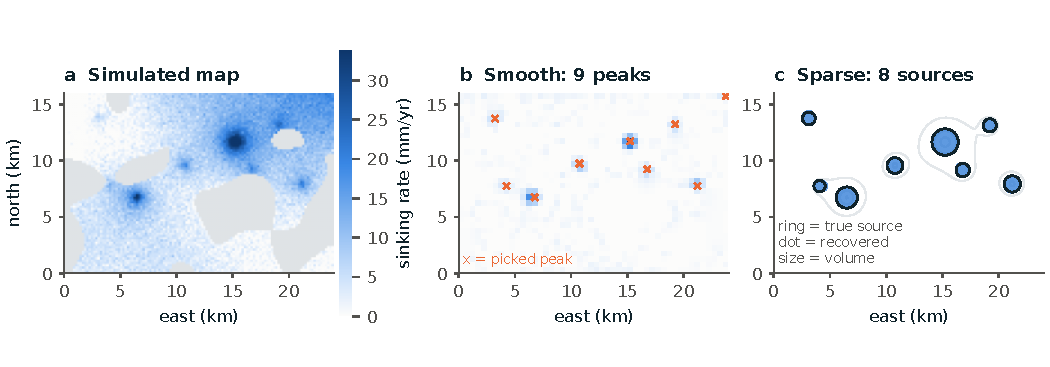
\includegraphics[width=\linewidth]{fig/example.pdf}
\caption{One of the \nScen\ maps. (a) What the radar would deliver; grey patches are missing data.
(b) The smooth baseline on its candidate grid. (c) The sparse result against the truth, with faint
contours of the true pumping signal. In this example both methods do well; across all maps the
smooth baseline produced \smNest\ peaks for \nTrue\ sources.}\label{fig:example}
\end{figure}

\subsection{Result 2: the uncertainty is honest}

\begin{itemize}
\item With $B$ known, \calCover\,\% of true volumes fall inside the stated 90\,\% range. That is
inside the 80--95\,\% band of check \V{7}.
\item The stability score separates real from false: its median is \calStabTp\ for true detections
and \calStabFp\ for false ones. Keeping only detections with stability of at least 0.8 raises
precision from \calPrecision\,\% to \calPrecisionStab\,\%, at the cost of recall falling from
\calRecall\,\% to \calRecallStab\,\%.
\item Small sources are not systematically missed: recall is \recallSmall\,\% for 40--80 \kcm,
\recallMid\,\% for 80--160 and \recallLarge\,\% for 160--400.
\end{itemize}

\begin{figure}[H]
\centering
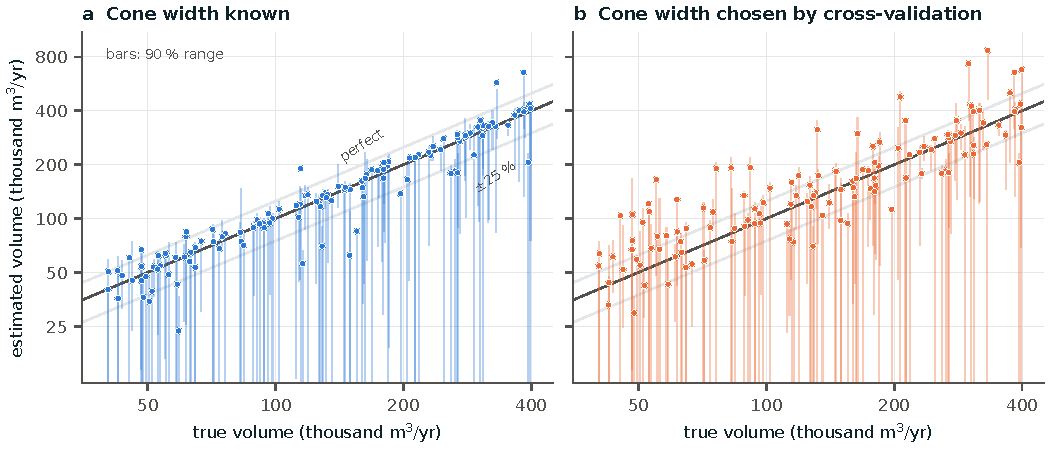
\includegraphics[width=\linewidth]{fig/volumes.pdf}
\caption{Estimated against true volume for every found source. (a) With the cone width known, points
hug the diagonal. (b) With the cone width chosen by cross-validation, whole maps shift up or down
together, because a wrong width rescales every source in that map.}\label{fig:volumes}
\end{figure}

\subsection{Result 3: where it breaks}

\begin{figure}[H]
\centering
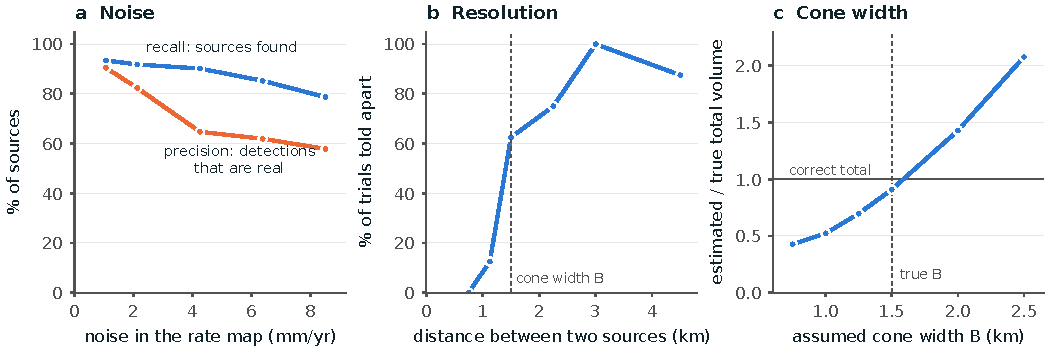
\includegraphics[width=\linewidth]{fig/limits.pdf}
\caption{Three limits, each from 8 maps per point with $B$ known in (a) and (b).
(a) More noise brings more false alarms. (b) Two equal sources of 200 \kcm\ are told apart only when
they are farther apart than about one cone width. (c) The estimated total volume grows with the
cone width that the analyst assumes.}\label{fig:limits}
\end{figure}

\textbf{Noise.} Table~\ref{tab:e2}. Recall stays high, but precision falls from \precNHalf\,\% at
\noiseHalf\,\mmyr\ to \precNTwo\,\% at \noiseTwo\,\mmyr. The stability filter becomes essential
there. Published Semarang maps report differences of 3--9\,\mmyr\ against GNSS \cite{azeriansyah2025,janur2025}, so careful quality control in \M{2} is
not optional.

\begin{table}[H]
\caption{Effect of noise ($B$ known).}\label{tab:e2}
\small\centering
\begin{tabular}{r r r r r}
\toprule
\textbf{Noise (\mmyr)} & \textbf{Recall (\%)} & \textbf{Precision (\%)} & \textbf{Volume error (\%)} & \textbf{Total}\\*
\midrule
\tabEtwo
\bottomrule
\end{tabular}
\end{table}

\textbf{Resolution.} Table~\ref{tab:e3}. Two sources closer than about one cone width (1.5\,km here)
are usually reported as one. The method resolves \emph{well fields}, not single wells. The merged
source still carries roughly the combined volume.

\begin{table}[H]
\caption{Telling two equal sources apart.}\label{tab:e3}
\small\centering
\begin{tabular}{r r r r}
\toprule
\textbf{Distance / $B$} & \textbf{Distance (km)} & \textbf{Told apart} & \textbf{Total}\\*
\midrule
\tabEthree
\bottomrule
\end{tabular}
\end{table}

\textbf{Cone width and shape.} Table~\ref{tab:e4}. This is the important one. If the analyst assumes
a cone half as wide as the true one, the total volume comes out at \totNarrow\ of the truth; with a
cone two-thirds wider, at \totWide. A Gaussian cone instead of the Bessel shape loses recall. In
contrast, detection is stable across widths from 1.0 to 2.5\,km (recall 85--86\,\%).

\begin{table}[H]
\caption{Effect of assuming the wrong cone (true: Bessel, $B = 1.5$\,km).}\label{tab:e4}
\small\centering
\begin{tabular}{l r r r r r}
\toprule
\textbf{Assumed shape} & \textbf{Width (km)} & \textbf{Recall (\%)} & \textbf{Precision (\%)} & \textbf{Volume error (\%)} & \textbf{Total}\\*
\midrule
\tabEfour
\bottomrule
\end{tabular}
\end{table}

\textbf{Can the data choose $B$ by itself?} Only roughly. Cross-validation picked the true 1.5\,km in
\cvBexact\ of \nScen\ maps and landed within 0.25\,km in \cvBnear. Its choices ranged from \cvBmin\ to
\cvBmax\,km. When it was right, the median volume error was \cvGoodErr\,\%; when it was wrong,
\cvBadErr\,\%. With $B$ from cross-validation, only \cvCover\,\% of true volumes fall inside the
stated range, below the pass band, because the bootstrap does not know that $B$ itself is uncertain.

\textbf{The ranking survives.} Even with a wrong cone width, the \emph{order} of sources is nearly
right. The rank correlation between true and estimated volumes is \rankCal\ with $B$ known, and
stays between \rankWide\ and \rankOneK\ for assumed widths from 0.75 to 2.5\,km.

\subsection{What we learned}

\begin{plain}
The inversion answers \emph{where} and \emph{in what order} reliably. It answers \emph{how much} only as
well as we know one number: the width of a pumping cone. So the audit should lead with the ranked
list, state volumes as a band across plausible cone widths, and narrow that band with well data.
\end{plain}

Four caveats about this experiment itself.
\begin{enumerate}
\item The same family of models made the data and inverted it. Table~\ref{tab:e4} relaxes this for
the cone, but not for everything else.
\item One cone width for the whole map. A real aquifer varies; a zoned $B$ is the natural extension.
\item Vertical motion was taken as given. Errors from stages \M{1}--\M{3} enter only as noise.
\item A snapshot in time. Sources that switch on or off (\M{4}) were not simulated.
\end{enumerate}

The code is in \texttt{code/}: \texttt{synth.py} (model and inversion), \texttt{run\_all.py} (the four
experiments), \texttt{analyze.py} (every number in this section) and \texttt{figures.py}.

\section{Feasibility}\label{sec:feas}

\begin{inshort}
The project is feasible with open data and a laptop. The measurement part is proven by earlier
studies. The inversion part works in simulation. The one real unknown is the cone width $B$, and
there are three ways to pin it down. A one-week test on real data settles the rest.
\end{inshort}

\Needspace{30\baselineskip}
\subsection{Verdict by component}

\Needspace{24\baselineskip}
{\small
\begin{xltabular}{\linewidth}{@{}L{36mm}L{22mm}Y@{}}
\toprule
\textbf{Component} & \textbf{Status} & \textbf{Evidence}\\*
\midrule
Radar time series, \M{1}--\M{3} & Proven & Four published Semarang studies used the same satellite
  \cite{lo2022,aditiya2023,azeriansyah2025,janur2025}; two used the same open tools.\\
Time-series separation, \M{4} & Low risk & Standard methods with published uses on radar data
  \cite{ebmeier2016,chaussard2014}.\\
Background model, \M{5} & Medium risk & Depends on a usable clay-thickness map (\D{7}). The smooth
  surface alone was enough in simulation.\\
Source inversion, \M{6} & Works in simulation & Section~\ref{sec:exp}: recall \calRecall\,\%, precision
  \calPrecision\,\%. Not yet run on real data.\\
Uncertainty, \M{7} & Works in simulation & Ranges cover \calCover\,\% of truths when $B$ is known.\\
Volume to extraction, \M{8} & Needs data & A lower bound is always available. An estimate needs \D{6}.\\
\bottomrule
\end{xltabular}}

\subsection{Pinning down the cone width}\label{sec:calB}

Section~\ref{sec:exp} showed that volumes scale with the assumed $B$. Three independent routes
constrain it. Using more than one is itself a check.

\begin{enumerate}
\item \textbf{Hydraulics.} $B=\sqrt{T\,b'/K'_v}$ (Eq.~\ref{eq:hantush}). Transmissivity $T$ comes from
pumping tests in well-completion reports; clay thickness $b'$ is 5--30\,m \cite{putranto2016}; clay
conductivity $K'_v$ from laboratory tests or model calibration \cite{lo2022}. This gives a range, not
a number.
\item \textbf{Water levels.} Where several monitoring wells surround a known well field, fit the
Bessel profile of Eq.~\eqref{eq:hantush} to their drawdowns.
\item \textbf{The radar map itself.} Find one isolated, clean bowl and fit $B$ to its shape alone.
A single clean source constrains the width far better than a crowded map does.
\end{enumerate}

Whatever the outcome, the audit reports each volume for a low, middle and high $B$, and leads with
the ranking, which is robust (rank correlation \rankWide--\rankCal\ in simulation).

\Needspace{29\baselineskip}
\subsection{One-week test on real data}\label{sec:spike}

Before the team commits six weeks, one person runs this test.

\Needspace{21\baselineskip}
{\small
\begin{xltabular}{\linewidth}{@{}L{16mm}Y@{}}
\toprule
\textbf{Day} & \textbf{Task}\\*
\midrule
1--2 & Download the LiCSAR frame for track 76, clip to Semarang--Demak, run LiCSBAS with GACOS.\\
3 & Compare the rate map with published ones: the north-east should exceed 80\,\mmyr\
  \cite{lo2022,aditiya2023}. Check the rate at the CSEM station.\\
4 & Convert to approximate vertical rates (one direction only, for the test). Build the cosine
  background.\\
5 & Run the inversion for $B$ = 1.0, 1.5 and 2.0\,km.\\
6 & Run the block bootstrap. Overlay sources on industrial land use.\\
7 & Decide.\\
\bottomrule
\end{xltabular}}

\textbf{Go if all four hold:}
\begin{itemize}
\item usable pixels cover at least half of the built-up and industrial land;
\item the rate map matches published maps in pattern and peak values;
\item at least five sources appear with stability of 0.8 or more, for all three values of $B$;
\item the map left over after the fit has a spread of 5\,\mmyr\ or less (earlier work reached 3.8
\cite{azeriansyah2025}).
\end{itemize}

\textbf{If not:} the radar products from days 1--3 are not wasted. They feed directly into two other
ideas from the shortlist that use the same maps: separating sea-level rise from land sinking, and
testing whether a groundwater ban slowed subsidence.

\Needspace{14\baselineskip}
\subsection{Risks}

\Needspace{8\baselineskip}
{\small
\begin{xltabular}{\linewidth}{@{}L{8mm}L{40mm}L{14mm}Y@{}}
\caption{Risk register.}\label{tab:risk}\\*
\toprule
 & \textbf{Risk} & \textbf{Level} & \textbf{Response}\\*
\midrule
\R{1} & Cone width $B$ is uncertain, so volumes can be off by a factor of about two either way. & High &
  Three calibration routes (Section~\ref{sec:calB}); report a band; lead with ranking.\\
\R{2} & Radar loses signal over fish ponds and rice fields, common in Demak. & High & State coverage
  honestly; add L-band data (\D{2}) as its record grows; lower resolution there.\\
\R{3} & Non-pumping subsidence is mistaken for pumping. & Medium & Background model \M{5} trained on quiet
  pixels; east--west motion and seasonal behaviour as extra evidence.\\
\R{4} & Groundwater records (\D{6}) are not released in time. & Medium & Ask in week 1. Without them, label
  results ``not yet checked against wells'' and rely on \V{1}--\V{4}.\\
\R{5} & Phase-unwrapping errors where the ground sinks fastest, worse in 2022--2024 when images came every
  12 days. & Medium & Loop-closure checks, short time gaps only, compare the two directions.\\
\R{6} & A step in the series where Sentinel-1A hands over to 1C and 1D. & Low & Process as one network across
  the April--June 2026 overlap; test for a jump at the hand-over.\\
\R{7} & Processing takes longer than planned. & Low & Start from ready-made LiCSAR pairs; clip to the study
  area; ascending track through on-demand processing.\\
\R{8} & Results are read as accusations against named companies. & Medium & See Section~\ref{sec:ethics}.\\
\bottomrule
\end{xltabular}}

\subsection{Responsible use}\label{sec:ethics}

The method points at places, and places have owners. Three rules keep it fair.

\begin{itemize}
\item \textbf{Hot spots, not names.} Public maps and the competition material show 500\,m cells and
land-use classes. Any link to a specific permit holder is for the regulator only.
\item \textbf{A lead, not a verdict.} A detected source is a reason to inspect a meter. It is not
proof of a violation: a permitted well field also makes a bowl.
\item \textbf{Say what the number is.} Every volume is labelled as lost storage and as a lower bound
on extraction, with its range and the assumed cone width.
\end{itemize}

\subsection{Computing needs}

A laptop with 16\,GB of memory is enough. The inversion and bootstrap for the test area take
minutes: one simulated map of 9,600 pixels and 1,536 candidates took under a minute on two cores.
The radar time series is the heavy step. Clipped to the study area and started from ready-made
pairs, we expect hours rather than days, but this is an estimate until the one-week test.

\clearpage\part{Software design}
\section{The product in brief}\label{sec:product}

\begin{inshort}
The research pipeline is wrapped in a small web application, working name \textbf{SUMUR} (Indonesian
for ``well''). An analyst starts a run; a regulator opens a map, reads a ranked list of extraction
hot spots, clicks one to see its evidence, and exports an audit sheet.
\end{inshort}

\Needspace{23\baselineskip}
\subsection{Users and what they need}

\Needspace{17\baselineskip}
{\small
\begin{xltabular}{\linewidth}{@{}L{38mm}Y@{}}
\toprule
\textbf{User} & \textbf{Question they bring}\\*
\midrule
Groundwater regulator (provincial energy office, Geological Agency) & ``Which sites should my inspectors
  visit first?''\\
Geospatial analyst (BIG, university) & ``Can I rerun this, check each step, and trust the numbers?''\\
City planner (planning and public-works offices) & ``How much sinking will remain even if pumping stops?''\\
Jury and public & ``What does this show, in two minutes?''\\
\bottomrule
\end{xltabular}}

\Needspace{24\baselineskip}
{\small
\begin{xltabular}{\linewidth}{@{}L{8mm}Y L{22mm}L{24mm}@{}}
\caption{User needs. Each one maps to research outputs and to software components.}\label{tab:needs}\\*
\toprule
 & \textbf{Need} & \textbf{Output} & \textbf{Component}\\*
\midrule
\U{1} & See where and how fast the ground sinks, with data gaps shown honestly. & \Ox{1} \Ox{2} & \Sx{7} \Sx{8}\\
\U{2} & Read a ranked list of hot spots with volume ranges and stability. & \Ox{3} & \Sx{7} \Sx{8}\\
\U{3} & Click a hot spot and see why it is there: time series, stability, land use, background share. & \Ox{3} \Ox{4} & \Sx{8}\\
\U{4} & Move the cone-width assumption and watch volumes change while the ranking holds. & \Ox{3} & \Sx{4} \Sx{8}\\
\U{5} & Export an audit sheet (PDF) and the data (GeoJSON, GeoTIFF). & \Ox{5} & \Sx{9}\\
\U{6} & Rerun when new satellite images arrive and see what changed. & all & \Sx{1} \Sx{5}\\
\bottomrule
\end{xltabular}}

\section{User flow}

\begin{figure}[H]
\centering
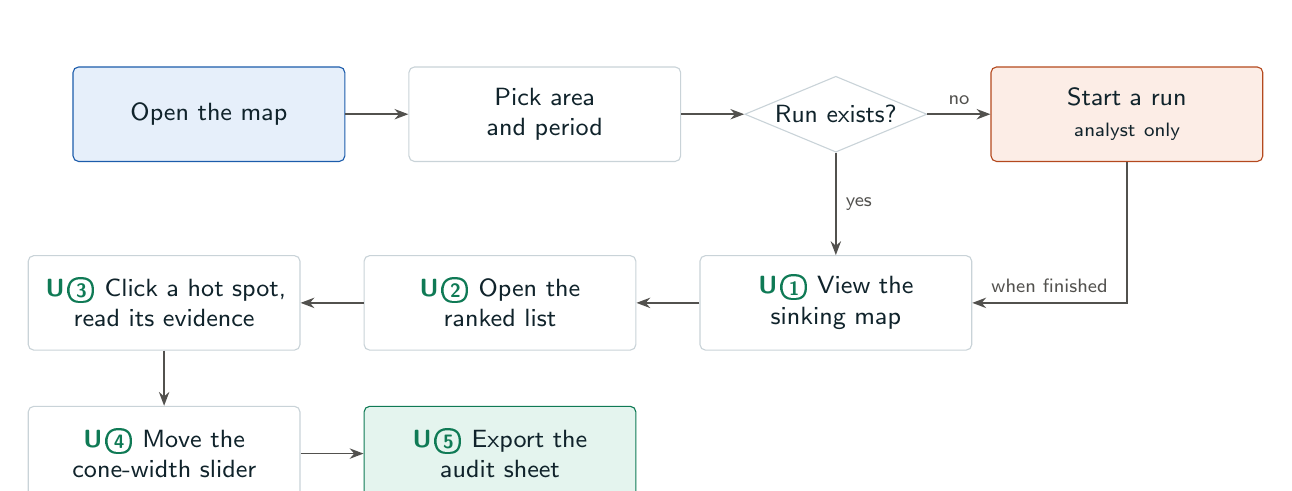
\begin{tikzpicture}[node distance=7mm and 8mm]
\tikzset{uf/.style={box,text width=31mm,minimum height=12mm}}
\node[uf,boxa] (a) {Open the map};
\node[uf,right=of a] (b) {Pick area\\and period};
\node[draw=line,diamond,aspect=2.4,inner sep=1pt,font=\sffamily\small,right=of b,text=ink] (c) {Run exists?};
\node[uf,boxw,right=of c] (d) {Start a run\\{\scriptsize analyst only}};
\node[uf,below=13mm of c] (e) {\U{1} View the\\sinking map};
\node[uf,left=of e] (f) {\U{2} Open the\\ranked list};
\node[uf,left=of f] (g) {\U{3} Click a hot spot,\\read its evidence};
\node[uf,below=of g] (h) {\U{4} Move the\\cone-width slider};
\node[uf,boxg,right=of h] (i) {\U{5} Export the\\audit sheet};
\draw[arr] (a)--(b); \draw[arr] (b)--(c);
\draw[arr] (c)-- node[lab,above]{no} (d);
\draw[arr] (c)-- node[lab,right]{yes} (e);
\draw[arr] (d.south) |- node[lab,pos=0.75,above]{when finished} (e.east);
\draw[arr] (e)--(f); \draw[arr] (f)--(g); \draw[arr] (g)--(h); \draw[arr] (h)--(i);
\end{tikzpicture}
\caption{The main path through the application. A regulator never starts a run; they open finished
ones.}\label{fig:userflow}
\end{figure}

\textbf{The evidence panel} (\U{3}) is where trust is won. For one hot spot it shows: the volume as a
band for low, middle and high cone width; the stability score; the displacement history of the
nearest pixels with change dates marked; the share of local sinking assigned to background; land use
under the source; and the match class from \M{9}.

\textbf{The cone-width slider} (\U{4}) is also the demonstration. Dragging it makes every volume grow
or shrink, while the order of the list barely moves. It shows the method's strength and its limit in
one gesture.

\section{Architecture}\label{sec:arch}

\begin{figure}[H]
\centering
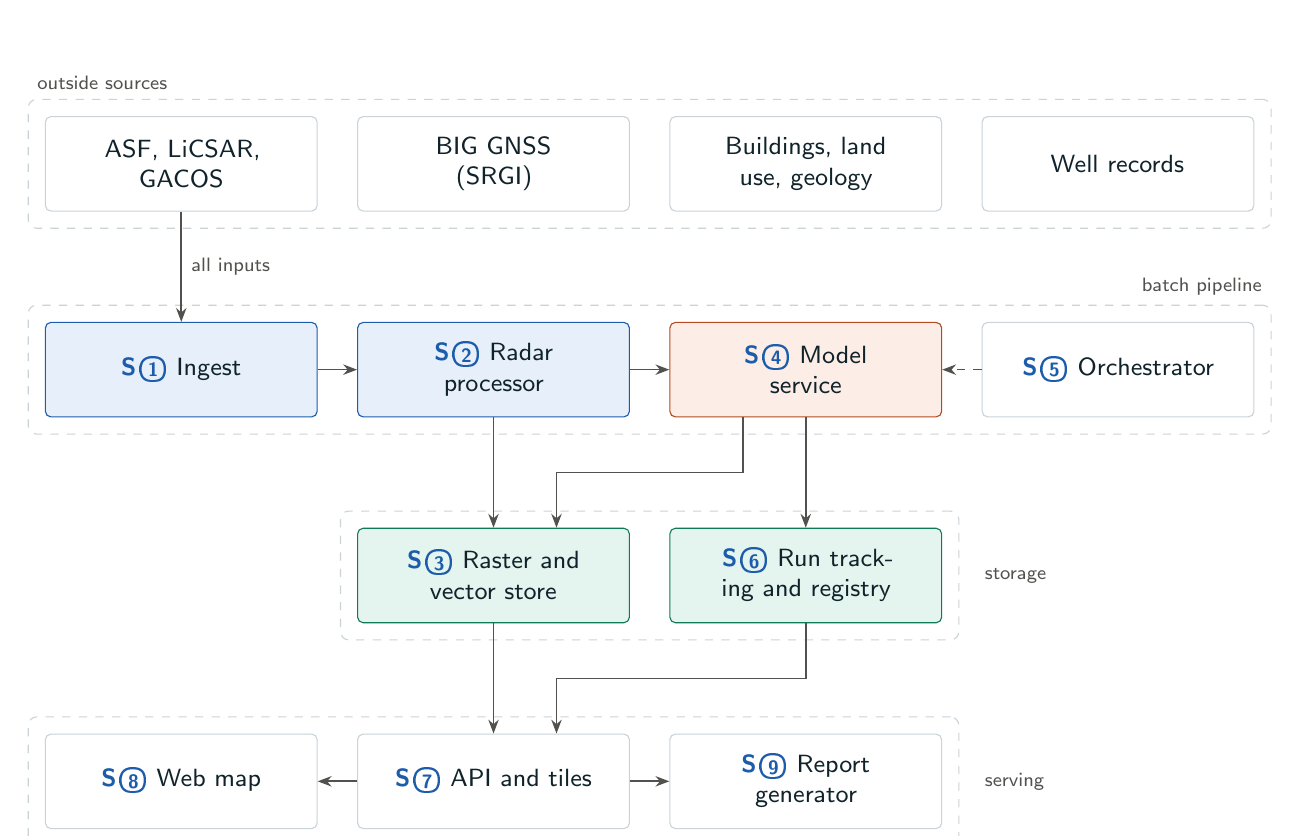
\begin{tikzpicture}[node distance=5mm and 5mm]
\tikzset{c/.style={box,text width=31mm,minimum height=12mm},
         band/.style={draw=line,dashed,rounded corners=3pt,inner sep=6pt}}
\node[c] (x1) {ASF, LiCSAR,\\GACOS};
\node[c,right=of x1] (x2) {BIG GNSS\\(SRGI)};
\node[c,right=of x2] (x3) {Buildings, land use, geology};
\node[c,right=of x3] (x4) {Well records};
\node[c,boxa,below=14mm of x1] (s1) {\Sx{1} Ingest};
\node[c,boxa,right=of s1] (s2) {\Sx{2} Radar\\processor};
\node[c,boxw,right=of s2] (s4) {\Sx{4} Model\\service};
\node[c,right=of s4] (s5) {\Sx{5} Orchestrator};
\node[c,boxg,below=14mm of s2] (s3) {\Sx{3} Raster and vector store};
\node[c,boxg,right=of s3] (s6) {\Sx{6} Run tracking and registry};
\node[c,below=14mm of s3] (s7) {\Sx{7} API and tiles};
\node[c,left=of s7] (s8) {\Sx{8} Web map};
\node[c,right=of s7] (s9) {\Sx{9} Report\\generator};
\begin{scope}[on background layer]
\node[band,fit=(x1)(x4)] (bx) {};
\node[band,fit=(s1)(s5)] (bp) {};
\node[band,fit=(s3)(s6)] (bst) {};
\node[band,fit=(s8)(s9)] (bsv) {};
\end{scope}
\node[lab,anchor=south west] at (bx.north west) {outside sources};
\node[lab,anchor=south east] at (bp.north east) {batch pipeline};
\node[lab,anchor=west] at ($(bst.east)+(2mm,0)$) {storage};
\node[lab,anchor=west] at ($(bsv.east)+(2mm,0)$) {serving};
\draw[arr] (x1.south)-- node[lab,right]{all inputs} (s1.north);
\draw[arr] (s1)--(s2); \draw[arr] (s2)--(s4);
\draw[arr,dashed] (s5)--(s4);
\draw[arr] (s2)--(s3); \draw[arr] (s4.south)--(s6.north);
\draw[arr] ([xshift=-8mm]s4.south)--++(0,-7mm)-|([xshift=8mm]s3.north);
\draw[arr] (s3)--(s7); \draw[arr] (s6.south)--++(0,-7mm)-|([xshift=8mm]s7.north);
\draw[arr] (s7)--(s8); \draw[arr] (s7)--(s9);
\end{tikzpicture}
\caption{Components and data flow. All outside data enter through \Sx{1}. The orchestrator \Sx{5}
schedules \Sx{1}, \Sx{2} and \Sx{4} and enforces the quality gates.}\label{fig:arch}
\end{figure}

\Needspace{8\baselineskip}
{\small
\begin{xltabular}{\linewidth}{@{}L{8mm}L{31mm}Y L{17mm}@{}}
\caption{Components.}\label{tab:components}\\*
\toprule
 & \textbf{Component} & \textbf{Responsibility} & \textbf{Stages}\\*
\midrule
\Sx{1} & Ingest & Find and download radar pairs, atmosphere maps, GNSS series, context layers. Record
  versions and hashes. & feeds \M{1}\\
\Sx{2} & Radar processor & Time series, quality control, referencing. Runs LiCSBAS and MintPy in
  containers. & \M{1} \M{2}\\
\Sx{3} & Raster and vector store & Displacement cubes and maps as cloud-friendly rasters; sources,
  runs and checks in a spatial database. & all\\
\Sx{4} & Model service & Decomposition, time-series separation, background model, inversion, bootstrap,
  volume conversion. Precomputes results for three cone widths. & \M{3}--\M{8}\\
\Sx{5} & Orchestrator & Runs the stages in order, retries failures, enforces quality gates. & all\\
\Sx{6} & Run tracking and registry & Stores settings, metrics and figures of every run; marks which
  run is published. & \V{1}--\V{7}\\
\Sx{7} & API and tiles & Serves runs, sources, time series and map tiles. & \M{9}\\
\Sx{8} & Web map & Map, ranked list, evidence panel, cone-width slider. & \M{9}\\
\Sx{9} & Report generator & Builds the audit sheet and data exports. & \M{9}\\
\bottomrule
\end{xltabular}}

\clearpage
\section{Sequence: running an audit}

\begin{figure}[H]
\centering
\resizebox{\linewidth}{!}{\sffamily\small
\begin{sequencediagram}
\newthread{u}{Analyst}
\newinst[1.5]{ui}{Web map}
\newinst[1.7]{api}{API}
\newinst[1.5]{orc}{Orchestrator}
\newinst[2.0]{wk}{Workers}
\newinst[1.5]{db}{Store}
\begin{call}{u}{Run}{ui}{map and list}
  \begin{call}{ui}{POST /audits}{api}{202, run id}
    \mess{api}{start run}{orc}
  \end{call}
  \postlevel
  \begin{sdblock}{loop}{until finished}
    \begin{call}{ui}{GET /audits/\{id\}}{api}{stage, progress}
    \end{call}
  \end{sdblock}
  \postlevel
  \begin{call}{orc}{radar: \M{1}--\M{2}}{wk}{gate 1 passed}
    \mess{wk}{cubes, masks}{db}
  \end{call}
  \postlevel
  \begin{call}{orc}{model: \M{3}--\M{8}}{wk}{gate 2 passed}
    \mess{wk}{sources, metrics}{db}
  \end{call}
  \postlevel
  \begin{call}{ui}{GET .../sources}{api}{GeoJSON}
    \begin{call}{api}{query}{db}{rows}
    \end{call}
  \end{call}
\end{call}
\end{sequencediagram}}
\caption{One audit run. Web map is \Sx{8}, API is \Sx{7}, orchestrator is \Sx{5}, workers are \Sx{1},
\Sx{2} and \Sx{4}, the store is \Sx{3} and \Sx{6}. The run is asynchronous: the web map polls for
progress while the orchestrator works (drawn one after the other here for readability). A failed
gate stops the run and reports which check failed.}\label{fig:seq}
\end{figure}

Two design choices keep the interface fast.
\begin{itemize}
\item \textbf{Nothing heavy on a click.} All maps are pre-rendered as tiles, and the inversion is
precomputed for low, middle and high cone width. The slider (\U{4}) only switches between stored
results.
\item \textbf{Runs are immutable.} A rerun with new data creates a new run. The interface can compare
two runs (\U{6}) because the old one is never overwritten.
\end{itemize}

\Needspace{36\baselineskip}
\section{The ML/AI pipeline in software}\label{sec:mlops}

\begin{inshort}
Every stage reads versioned inputs and writes versioned outputs. Three quality gates decide whether a
run may continue or be published. A synthetic benchmark runs on every code change.
\end{inshort}

\Needspace{28\baselineskip}
{\small
\begin{xltabular}{\linewidth}{@{}L{17mm}L{35mm}L{37mm}Y@{}}
\caption{Pipeline stages as software steps.}\label{tab:dag}\\*
\toprule
\textbf{Stages} & \textbf{Reads} & \textbf{Writes} & \textbf{Key settings}\\*
\midrule
\M{1} \M{2} & Radar pairs, atmosphere maps, GNSS & Displacement cubes, mask, per-pixel uncertainty &
  Pair network, coherence threshold, reference station\\
\M{3} & Two cubes & Vertical and east--west cubes & Viewing angles\\
\M{4} & Vertical cube, rainfall & Rate, seasonal and change-date maps & Loss function, number of
  components, change penalty\\
\M{5} & Rate map, context layers & Background map, driver model, SHAP tables & Quiet-pixel distance, tree
  settings\\
\M{6} & Rate map, background & Source list per cone width & Candidate spacing, kernel family, $B$ values,
  penalty floor percentile\\
\M{7} & As \M{6} & Ranges and stability & Block size, number of resamples\\
\M{8} \M{9} & Sources, well records, land use & Audit list, report & Calibration set, match radius\\
\bottomrule
\end{xltabular}}

\Needspace{21\baselineskip}
\subsection{Quality gates}

\Needspace{15\baselineskip}
{\small
\begin{xltabular}{\linewidth}{@{}L{17mm}L{28mm}Y Y@{}}
\toprule
\textbf{Gate} & \textbf{After} & \textbf{Must pass} & \textbf{If it fails}\\*
\midrule
Gate 1 & \M{2} & \V{1} radar against GNSS; \V{2} loop closure & Stop. Fix pair network or masks.\\
Gate 2 & \M{7} & \V{3} synthetic benchmark with this run's noise level and data gaps; \V{4} out-of-sample
  fit & Stop. Report which metric failed.\\
Gate 3 & Before publishing & \V{7} range coverage; \V{5} and \V{6} if well data exist; sign-off by a named
  analyst & Keep the run private.\\
\bottomrule
\end{xltabular}}

Gate 2 deserves a note. The synthetic benchmark is rerun \emph{with the real run's own noise level
and data-gap pattern}. Section~\ref{sec:exp} showed that precision depends on noise. A run over a
noisy area therefore gets its own, honest expectation of how many detections are real.

\subsection{Versioning and tracking}

\begin{itemize}
\item \textbf{One identity per run:} code commit, configuration hash and input-data hashes. Two runs
with the same three give the same outputs (fixed seeds).
\item \textbf{Data versioning} with DVC: large files live in object storage; small pointer files live
in the repository.
\item \textbf{Run tracking} with MLflow: settings, the metrics of Table~\ref{tab:valid}, and
diagnostic figures for every run.
\item \textbf{Model card and data card} shipped with each published run: what it is for, what it must
not be used for, known limits (Sections~\ref{sec:exp} and~\ref{sec:ethics}).
\end{itemize}

\Needspace{27\baselineskip}
\subsection{Tests}

\Needspace{21\baselineskip}
{\small
\begin{xltabular}{\linewidth}{@{}L{30mm}Y@{}}
\toprule
\textbf{Kind} & \textbf{Examples}\\*
\midrule
Unit & The kernel integrates to one. Line-of-sight vectors have unit length. Decomposition recovers a
  known vertical motion.\\
Property & Source volumes are never negative. Doubling the input map doubles the volumes. Shifting the
  map shifts the sources.\\
Regression & The synthetic benchmark of Section~\ref{sec:exp} on a fixed seed set must keep recall and
  precision at 80\,\% or more and median volume error at 25\,\% or less.\\
Data & Coordinate systems match. No-data values are consistent. Fewer than 5\,\% of pairs fail loop
  closure.\\
End to end & A ten-image sample runs from download to audit sheet in the build pipeline.\\
\bottomrule
\end{xltabular}}

\subsection{Staying current}

Sentinel-1 now revisits every 6 days \cite{s1status}. The orchestrator checks for new images weekly
and proposes a rerun monthly. Each rerun is compared with the previous one: a source whose volume
range no longer overlaps its earlier range is flagged as changed. Drift checks (residual spread,
difference from GNSS) run on every update and raise an alert when they leave their usual band.

\Needspace{30\baselineskip}
\section{Data model and API}

\Needspace{24\baselineskip}
{\small
\begin{xltabular}{\linewidth}{@{}L{31mm}Y@{}}
\caption{Main tables in the spatial database.}\label{tab:datamodel}\\*
\toprule
\textbf{Table} & \textbf{Key fields}\\*
\midrule
\texttt{audit\_run} & id, area, period, code commit, configuration hash, data hashes, status, gate results,
  published flag, signed-off by\\
\texttt{raster\_asset} & run id, layer name (vertical rate, seasonal amplitude, background, \ldots), file
  location, resolution, statistics\\
\texttt{source} & id, run id, position, 500\,m cell, stability, match class, land-use class\\
\texttt{source\_estimate} & source id, cone width, volume, 5th and 95th percentile, rank\\
\texttt{validation\_result} & run id, check (\V{1}--\V{7}), value, pass mark, passed\\
\texttt{well\_record} & restricted: position, depth, permitted volume, head series; calibration or
  validation set\\
\bottomrule
\end{xltabular}}

\Needspace{27\baselineskip}
{\small
\begin{xltabular}{\linewidth}{@{}L{58mm}Y L{12mm}@{}}
\caption{API endpoints.}\label{tab:api}\\*
\toprule
\textbf{Endpoint} & \textbf{Returns} & \textbf{Need}\\*
\midrule
\texttt{POST /audits} & Starts a run for an area and period; returns a run id. Analysts only. & \U{6}\\
\texttt{GET /audits/\{id\}} & Status, current stage, gate results. & \U{6}\\
\texttt{GET /audits/\{id\}/sources?b=mid} & Ranked sources as GeoJSON for the chosen cone width. & \U{2} \U{4}\\
\texttt{GET /sources/\{id\}} & One source with all three estimates and its evidence. & \U{3}\\
\texttt{GET /sources/\{id\}/timeseries} & Displacement history of nearby pixels, with change dates. & \U{3}\\
\texttt{GET /tiles/\{layer\}/\{z\}/\{x\}/\{y\}} & Map tiles for any raster layer. & \U{1}\\
\texttt{GET /audits/\{id\}/report.pdf} & The audit sheet. & \U{5}\\
\texttt{GET /audits/\{a\}/compare/\{b\}} & Sources that appeared, vanished or changed between two runs. & \U{6}\\
\bottomrule
\end{xltabular}}

One source, as the API returns it:

{\small
\begin{verbatim}
{ "type": "Feature",
  "geometry": { "type": "Point", "coordinates": [110.46, -6.95] },
  "properties": {
    "rank": 3, "cell": "SMG-0412", "stability": 0.93,
    "volume_m3_per_yr": { "low_B": 61000, "mid_B": 118000, "high_B": 171000 },
    "range_90_mid_B": [84000, 149000],
    "meaning": "lost storage; lower bound on extraction",
    "background_share": 0.22, "land_use": "industrial",
    "match": "no permit on record nearby" } }
\end{verbatim}
}
The values above are placeholders that show the format. They are not results.

\Needspace{14\baselineskip}
\section{Technology choices}

\Needspace{8\baselineskip}
{\small
\begin{xltabular}{\linewidth}{@{}L{27mm}L{45mm}Y L{9mm}@{}}
\caption{Stack. ``First'' marks what the six-week build needs.}\label{tab:stack}\\*
\toprule
\textbf{Layer} & \textbf{Choice} & \textbf{Why} & \textbf{First}\\*
\midrule
Radar processing & LiCSAR pairs with LiCSBAS; ASF on-demand pairs with MintPy; GACOS & Open, documented,
  already used on Semarang & yes\\
Numerics & Python, NumPy, SciPy, scikit-learn, xarray, rasterio, GeoPandas & The inversion in this report
  already runs on them & yes\\
Learning & LightGBM or XGBoost, SHAP, \texttt{ruptures} for change points & Small, explainable models & yes\\
Orchestration & DVC pipeline first; Prefect later & One command reruns everything; scheduling can wait & yes\\
Storage & Cloud-optimised GeoTIFF and Zarr; PostgreSQL with PostGIS & Standard, tile-friendly, queryable & yes\\
API and tiles & FastAPI; TiTiler & Typed, fast, serves rasters without pre-cutting tiles & yes\\
Web map & MapLibre GL JS with deck.gl & Open, handles rasters and thousands of points smoothly & yes\\
Tracking & MLflow; DVC & Every number traceable to a run & yes\\
Packaging & Docker and Docker Compose & The same environment on every laptop & yes\\
Build pipeline & GitHub Actions with pytest & The synthetic benchmark guards every change & yes\\
Report & HTML template rendered to PDF & Same content as the web panel & later\\
Extra data & NISAR L-band; ALOS-2 & Better over vegetation and ponds & later\\
\bottomrule
\end{xltabular}}

Repository layout:

{\small
\begin{verbatim}
sumur/
  config/         one YAML file per study area
  pipeline/       ingest.py  insar.py  decompose.py  separate.py
                  background.py  invert.py  uncertainty.py  attribute.py
  synth/          forward model and benchmark (the code shipped with this report)
  api/            FastAPI application
  web/            map, ranked list, evidence panel
  tests/          unit, property, regression, data, end-to-end
  dvc.yaml        the stage graph        docker-compose.yml
\end{verbatim}
}

\section{Quality attributes}

\begin{itemize}
\item \textbf{Reproducible.} One command rebuilds a run from raw inputs.
\item \textbf{Honest by design.} No volume is shown without its range, its cone-width band and the
words ``lower bound''. Data gaps are drawn as gaps, never interpolated silently.
\item \textbf{Fast to read.} The map and list load in about two seconds on a normal connection.
\item \textbf{Restricted where needed.} Well records and permit matches sit behind a login. Public
views show cells and classes only.
\item \textbf{Bilingual.} Indonesian and English interface and audit sheet.
\item \textbf{Portable.} Changing the study area means changing one configuration file. The same
build can be pointed at Pekalongan, Jakarta, Bangkok or the Mekong delta.
\end{itemize}

\Needspace{30\baselineskip}
\section{Build plan and competition fit}\label{sec:plan}

\Needspace{24\baselineskip}
{\small
\begin{xltabular}{\linewidth}{@{}L{14mm}Y L{37mm}@{}}
\caption{Six weeks. Confirm the national deadline with BIG before fixing dates.}\label{tab:plan}\\*
\toprule
\textbf{Week} & \textbf{Work} & \textbf{Done when}\\*
\midrule
1 & One-week test (Section~\ref{sec:spike}). Send data requests for \D{4} and \D{6}. & Go or no-go decided\\
2 & Both radar directions processed; vertical and east--west maps; GNSS check. & Gate 1 passes\\
3 & Time-series separation; background model; inversion and bootstrap on real data. & Gate 2 passes\\
4 & Calibrate cone width; well checks if data arrived; API and web map with real results. & Evidence panel
  works for every source\\
5 & Slides in English; two-minute video; audit sheet. & Dry run of the 10-minute talk\\
6 & Forms and letters; buffer; submit. & Submitted\\
\bottomrule
\end{xltabular}}

\textbf{Roles for a team of four.} Radar lead (\M{1}--\M{3}, \Sx{2}). Modelling lead (\M{4}--\M{8},
\Sx{4}, the benchmark). Software lead (\Sx{3}, \Sx{5}--\Sx{9}). Story and data lead (data requests,
\M{9}, slides, video, team representative).

\Needspace{23\baselineskip}
{\small
\begin{xltabular}{\linewidth}{@{}L{46mm}L{13mm}Y@{}}
\caption{How the work scores against the official judging weights.}\label{tab:agc}\\*
\toprule
\textbf{Criterion} & \textbf{Weight} & \textbf{What earns the points}\\*
\midrule
Challenge statement and relevance & 20\,\% & A named coast, a measured problem, and three goals:
  sustainable water use (SDG 6.4), safer cities (SDG 11.5) and climate resilience (SDG 13.1).\\
Application of geospatial technology & 40\,\% & Two-direction radar tied to BIG's own GNSS network; a
  physics-based sparse inversion; tested uncertainty; open benchmark.\\
Communication and storytelling & 20\,\% & One image: a sinking bowl resolves into a few points on
  factory roofs, each with a number and an error bar.\\
Creativity and originality & 20\,\% & First ranked, uncertainty-aware source list for an Indonesian
  city, built without a well registry; honest about its own limit.\\
\bottomrule
\end{xltabular}}

\clearpage\part{Traceability and references}
\Needspace{28\baselineskip}
\section{Traceability}\label{sec:trace}

\begin{inshort}
Read a row from left to right to follow one thread: from a question, through the data and method
that answer it, to the check that tests it, the software that runs it and the output that delivers
it.
\end{inshort}

\Needspace{16\baselineskip}
{\small
\begin{xltabular}{\linewidth}{@{}L{21mm}L{25mm}L{25mm}L{25mm}L{22mm}Y@{}}
\caption{From research question to delivered output.}\label{tab:traceq}\\*
\toprule
\textbf{Question} & \textbf{Data} & \textbf{Method} & \textbf{Validation} & \textbf{Software} & \textbf{Output}\\*
\midrule
\Q{1} How fast? & \D{1} \D{2} \D{3} \D{4} \D{5} & \M{1} \M{2} \M{3} \M{4} & \V{1} \V{2} \V{4} & \Sx{1} \Sx{2} \Sx{3} & \Ox{1} \Ox{2}\\
\Q{2} Which sources, how much? & \D{6} \D{8} and the maps from \Q{1} & \M{6} \M{7} \M{8} \M{9} & \V{3} \V{5} \V{6} \V{7} & \Sx{4} \Sx{7} \Sx{8} \Sx{9} & \Ox{3} \Ox{5}\\
\Q{3} How much is not pumping? & \D{5} \D{7} \D{8} \D{9} & \M{4} \M{5} & \V{4} & \Sx{4} & \Ox{2} \Ox{4}\\
\bottomrule
\end{xltabular}}

\Needspace{26\baselineskip}
{\small
\begin{xltabular}{\linewidth}{@{}L{46mm}L{24mm}L{24mm}L{22mm}Y@{}}
\caption{Each method stage with its inputs, checks, software home and main risks.}\label{tab:tracem}\\*
\toprule
\textbf{Stage} & \textbf{Data} & \textbf{Checked by} & \textbf{Runs in} & \textbf{Risks}\\*
\midrule
\M{1} Radar time series & \D{1} \D{2} \D{5} & \V{2} & \Sx{1} \Sx{2} & \R{5} \R{6} \R{7}\\
\M{2} Quality control & \D{3} \D{4} & \V{1} \V{2} & \Sx{2} & \R{2} \R{5}\\
\M{3} Vertical / east--west & from \M{2} & \V{1} & \Sx{4} & \\
\M{4} Time-series separation & \D{9} & \V{4} & \Sx{4} & \R{3}\\
\M{5} Background model & \D{5} \D{7} \D{8} & \V{4} & \Sx{4} & \R{3}\\
\M{6} Sparse source inversion & from \M{3}--\M{5} & \V{3} \V{5} \V{6} & \Sx{4} & \R{1}\\
\M{7} Uncertainty & from \M{6} & \V{7} & \Sx{4} & \R{1}\\
\M{8} Volume to extraction & \D{6} & \V{5} & \Sx{4} & \R{1} \R{4}\\
\M{9} Attribution and ranking & \D{6} \D{8} & \V{6} & \Sx{7} \Sx{8} \Sx{9} & \R{8}\\
\bottomrule
\end{xltabular}}

\Needspace{24\baselineskip}
{\small
\begin{xltabular}{\linewidth}{@{}L{44mm}L{34mm}Y@{}}
\caption{Status of each validation check today.}\label{tab:tracev}\\*
\toprule
\textbf{Check} & \textbf{Status} & \textbf{Where}\\*
\midrule
\V{1} Radar against GNSS & Planned, week 2 & Needs \D{4}\\
\V{2} Internal consistency & Planned, weeks 1--2 & One-week test, Section~\ref{sec:spike}\\
\V{3} Synthetic recovery & \textbf{Done}: passed with $B$ known & Section~\ref{sec:exp}, Table~\ref{tab:e1}\\
\V{4} Out-of-sample fit & Planned, week 3 & Needs real maps\\
\V{5} Wells: heads & Planned, week 4 & Needs \D{6}\\
\V{6} Wells: locations & Planned, week 4 & Needs \D{6}\\
\V{7} Honest ranges & \textbf{Done}: \calCover\,\% coverage with $B$ known; \cvCover\,\% without & Section~\ref{sec:exp}\\
\bottomrule
\end{xltabular}}

User needs \U{1}--\U{6} are traced to outputs and components in Table~\ref{tab:needs}.

\section{Glossary}

\begin{description}[leftmargin=34mm,style=nextline,font=\sffamily\bfseries\small,itemsep=1pt]
\item[Aquifer / aquitard] A layer that yields water (sand, gravel) / a layer that barely lets water through (clay).
\item[Confined aquifer] An aquifer sealed under clay, so its water is under pressure.
\item[Head] The level water rises to in a well; a measure of water pressure.
\item[Drawdown; pumping cone] The fall in head caused by pumping; it is deepest at the well and fades with distance, forming a cone.
\item[Cone width $B$] The distance over which a pumping cone fades (the leakage factor).
\item[Compaction] Squeezing of clay when water pressure falls. Mostly permanent.
\item[Lost storage] The volume by which the aquifer system has shrunk. Equal to the volume of the subsidence bowl.
\item[InSAR] Measuring ground motion by comparing the phase of radar images taken at different times.
\item[Line of sight] The direction from ground to satellite. One radar pass sees only motion along it.
\item[Ascending / descending] The satellite flying north or south. The two give two viewing directions.
\item[Coherence] How well a pixel keeps its radar signature over time. Water and crops lose it.
\item[SBAS] A way of building a displacement history from many pairs of images taken close together in time.
\item[GNSS / CORS] Satellite positioning (GPS and others) / a permanent station that records its position continuously.
\item[Sparse inversion] Finding the few causes that explain a measured pattern, instead of a smooth map of many small ones.
\item[Lasso] A regression that adds a penalty which pushes most coefficients to exactly zero.
\item[Bootstrap] Re-running an analysis on resampled data to see how much the answer varies.
\item[Stability] The share of bootstrap reruns in which a source reappears.
\item[Recall / precision] The share of true sources that were found / the share of detections that are real.
\item[Cross-validation] Testing a model on data held back from fitting. In blocks, because neighbouring pixels are alike.
\item[SHAP] A method that splits a model's prediction into contributions from each input.
\end{description}

\begin{thebibliography}{99}\small\raggedright
\bibitem{abidin2013} H.Z. Abidin, H. Andreas, I. Gumilar, T.P. Sidiq, Y. Fukuda. Land subsidence in coastal city of Semarang (Indonesia): characteristics, impacts and causes. \emph{Geomatics, Natural Hazards and Risk} 4(3), 226--240, 2013.
\bibitem{aditiya2023} A. Aditiya, T. Ito. Present-day land subsidence over Semarang revealed by time series InSAR new small baseline subset technique. \emph{Int.\ J.\ Applied Earth Observation and Geoinformation} 125, 103579, 2023. \url{https://doaj.org/article/bc659cefcb624b38a679829477d8e2d1}
\bibitem{aghnia2022} S. Aghnia, H. Hendrayana, D.P.E. Putra. Characteristics and potential of confined aquifers in Genuk and surrounding area, Semarang City. \emph{Proc.\ ICOSEAT 2022}. doi:10.2991/978-94-6463-086-2\_87
\bibitem{anantrasirichai2018} N. Anantrasirichai, J. Biggs, F. Albino, P. Hill, D. Bull. Application of machine learning to classification of volcanic deformation in routinely generated InSAR data. \emph{J.\ Geophys.\ Res.\ Solid Earth} 123, 6592--6606, 2018.
\bibitem{azeriansyah2025} R. Azeriansyah, K.-E. Ching, B.D. Yuwono. Impact of land subsidence-induced three-dimensional surface deformation on infrastructure in the Semarang--Demak alluvial plain, Indonesia. \emph{J.\ Earth and Marine Technology} 5(2), 111--122, 2025. \url{https://ejournal.itats.ac.id/jemt/article/download/6841/4469}
\bibitem{berardino2002} P. Berardino, G. Fornaro, R. Lanari, E. Sansosti. A new algorithm for surface deformation monitoring based on small baseline differential SAR interferograms. \emph{IEEE Trans.\ Geosci.\ Remote Sens.} 40(11), 2375--2383, 2002.
\bibitem{chaussard2013} E. Chaussard, F. Amelung, H. Abidin, S.-H. Hong. Sinking cities in Indonesia: ALOS PALSAR detects rapid subsidence due to groundwater and gas extraction. \emph{Remote Sensing of Environment} 128, 150--161, 2013.
\bibitem{chaussard2014} E. Chaussard, R. B\"urgmann, M. Shirzaei, E.J. Fielding, B. Baker. Predictability of hydraulic head changes and characterization of aquifer-system and fault properties from InSAR-derived ground deformation. \emph{J.\ Geophys.\ Res.\ Solid Earth} 119, 6572--6590, 2014.
\bibitem{chen2016} T. Chen, C. Guestrin. XGBoost: a scalable tree boosting system. \emph{Proc.\ KDD}, 2016.
\bibitem{ebmeier2016} S.K. Ebmeier. Application of independent component analysis to multitemporal InSAR data with volcanic case studies. \emph{J.\ Geophys.\ Res.\ Solid Earth} 121, 8970--8986, 2016.
\bibitem{esdm2023} Ministry of Energy and Mineral Resources. Press release 652.Pers/04/SJI/2023 on the amendment of the groundwater-approval decree, 21 December 2023. \url{https://esdm.go.id/en/media-center/news-archives/kementerian-esdm-lakukan-penyesuaian-kepmen-penyelenggaraan-persetujuan-penggunaan-air-tanah-}
\bibitem{fahrudin2012} Fahrudin, Najib. Study of the piezometric surface and hydrocompaction at confined aquifer caused the land subsidence in Semarang. \emph{Teknik} 32(1), 72--78, 2012.
\bibitem{frontiers2023} Cost--benefit study of replacing groundwater abstraction wells in Semarang--Demak. \emph{Frontiers in Environmental Economics}, 2023. doi:10.3389/frevc.2023.1073089
\bibitem{galloway2011} D.L. Galloway, T.J. Burbey. Review: regional land subsidence accompanying groundwater extraction. \emph{Hydrogeology Journal} 19, 1459--1486, 2011.
\bibitem{geertsma1973} J. Geertsma. Land subsidence above compacting oil and gas reservoirs. \emph{J.\ Petroleum Technology} 25(6), 734--744, 1973.
\bibitem{hantush1955} M.S. Hantush, C.E. Jacob. Non-steady radial flow in an infinite leaky aquifer. \emph{Trans.\ American Geophysical Union} 36(1), 95--100, 1955.
\bibitem{hoffmann2001} J. Hoffmann, H.A. Zebker, D.L. Galloway, F. Amelung. Seasonal subsidence and rebound in Las Vegas Valley, Nevada, observed by synthetic aperture radar interferometry. \emph{Water Resources Research} 37(6), 1551--1566, 2001.
\bibitem{hyvarinen2000} A. Hyv\"arinen, E. Oja. Independent component analysis: algorithms and applications. \emph{Neural Networks} 13, 411--430, 2000.
\bibitem{janur2025} A. Janur, Harintaka, A.G. Suhadha. Uneven land subsidence patterns along Java's northern urban corridor (Pantura route) from 2.5D SBAS InSAR approach. \emph{Indonesian J.\ on Geoscience} 12(2), 281--300, 2025. doi:10.17014/ijog.12.2.281-300
\bibitem{kepmen291} Ministry of Energy and Mineral Resources. Decree 291.K/GL.01/MEM.G/2023 on standards for groundwater-use approval; press release 529.Pers/04/SJI/2023, 4 November 2023. \url{https://www.esdm.go.id/id/media-center/arsip-berita/jangan-khawatir-sebagian-besar-rumah-tangga-tidak-perlu-izin-air-tanah}
\bibitem{killick2012} R. Killick, P. Fearnhead, I.A. Eckley. Optimal detection of changepoints with a linear computational cost. \emph{J.\ American Statistical Association} 107, 1590--1598, 2012.
\bibitem{lo2022} W. Lo, S.N. Purnomo, B.G. Dewanto, D. Sarah, Sumiyanto. Integration of numerical models and InSAR techniques to assess land subsidence due to excessive groundwater abstraction in the coastal and lowland regions of Semarang City. \emph{Water} 14(2), 201, 2022. \url{https://www.mdpi.com/2073-4441/14/2/201}
\bibitem{lundberg2017} S.M. Lundberg, S.-I. Lee. A unified approach to interpreting model predictions. \emph{Advances in Neural Information Processing Systems} 30, 2017.
\bibitem{meinshausen2010} N. Meinshausen, P. B\"uhlmann. Stability selection. \emph{J.\ Royal Statistical Society B} 72, 417--473, 2010.
\bibitem{mogi1958} K. Mogi. Relations between the eruptions of various volcanoes and the deformations of the ground surfaces around them. \emph{Bull.\ Earthquake Research Institute} 36, 99--134, 1958.
\bibitem{morishita2020} Y. Morishita, M. Lazecky, T.J. Wright, J.R. Weiss, J.R. Elliott, A. Hooper. LiCSBAS: an open-source InSAR time series analysis package integrated with the LiCSAR automated Sentinel-1 InSAR processor. \emph{Remote Sensing} 12(3), 424, 2020.
\bibitem{nisar2026} Alaska Satellite Facility. NISAR data availability overview, 2026. \url{https://nisar-docs.asf.alaska.edu/availability-overview/}
\bibitem{putranto2016} T.T. Putranto, T.R. R\"ude. Hydrogeological model of an urban city in a coastal area, case study: Semarang, Indonesia. \emph{Indonesian J.\ on Geoscience} 3(1), 17--27, 2016. \url{https://ijog.geologi.esdm.go.id/index.php/IJOG/article/view/227}
\bibitem{roberts2017} D.R. Roberts et al. Cross-validation strategies for data with temporal, spatial, hierarchical, or phylogenetic structure. \emph{Ecography} 40, 913--929, 2017.
\bibitem{ronneberger2015} O. Ronneberger, P. Fischer, T. Brox. U-Net: convolutional networks for biomedical image segmentation. \emph{Proc.\ MICCAI}, 2015.
\bibitem{s1status} Copernicus Data Space Ecosystem. S1C/D final orbital configuration achieved, 24 June 2026, \url{https://dataspace.copernicus.eu/node/4010}; ASF HyP3 documentation, Sentinel-1 mission, \url{https://hyp3-docs.asf.alaska.edu/sentinel1/}
\bibitem{smith2017} R.G. Smith, R. Knight, J. Chen, J.A. Reeves, H.A. Zebker, T. Farr, Z. Liu. Estimating the permanent loss of groundwater storage in the southern San Joaquin Valley, California. \emph{Water Resources Research} 53, 2133--2148, 2017.
\bibitem{tibshirani1996} R. Tibshirani. Regression shrinkage and selection via the lasso. \emph{J.\ Royal Statistical Society B} 58, 267--288, 1996.
\bibitem{vasco2019} D.W. Vasco, T.G. Farr, P. Jeanne, C. Doughty, P. Nico. Satellite-based monitoring of groundwater depletion in California's Central Valley. \emph{Scientific Reports} 9, 16053, 2019. doi:10.1038/s41598-019-52371-7
\bibitem{wright2004} T.J. Wright, B.E. Parsons, Z. Lu. Toward mapping surface deformation in three dimensions using InSAR. \emph{Geophysical Research Letters} 31, L01607, 2004.
\bibitem{yu2018} C. Yu, Z. Li, N.T. Penna, P. Crippa. Generic atmospheric correction model for interferometric synthetic aperture radar observations. \emph{J.\ Geophys.\ Res.\ Solid Earth} 123, 9202--9222, 2018.
\bibitem{yunjun2019} Z. Yunjun, H. Fattahi, F. Amelung. Small baseline InSAR time series analysis: unwrapping error correction and noise reduction. \emph{Computers \& Geosciences} 133, 104331, 2019.
\end{thebibliography}

\end{document}
